\documentclass[1p]{elsarticle_modified}
%\bibliographystyle{elsarticle-num}

%\usepackage[colorlinks]{hyperref}
%\usepackage{abbrmath_seonhwa} %\Abb, \Ascr, \Acal ,\Abf, \Afrak
\usepackage{amsfonts}
\usepackage{amssymb}
\usepackage{amsmath}
\usepackage{amsthm}
\usepackage{scalefnt}
\usepackage{amsbsy}
\usepackage{kotex}
\usepackage{caption}
\usepackage{subfig}
\usepackage{color}
\usepackage{graphicx}
\usepackage{xcolor} %% white, black, red, green, blue, cyan, magenta, yellow
\usepackage{float}
\usepackage{setspace}
\usepackage{hyperref}

\usepackage{tikz}
\usetikzlibrary{arrows}

\usepackage{multirow}
\usepackage{array} % fixed length table
\usepackage{hhline}

%%%%%%%%%%%%%%%%%%%%%
\makeatletter
\renewcommand*\env@matrix[1][\arraystretch]{%
	\edef\arraystretch{#1}%
	\hskip -\arraycolsep
	\let\@ifnextchar\new@ifnextchar
	\array{*\c@MaxMatrixCols c}}
\makeatother %https://tex.stackexchange.com/questions/14071/how-can-i-increase-the-line-spacing-in-a-matrix
%%%%%%%%%%%%%%%

\usepackage[normalem]{ulem}

\newcommand{\msout}[1]{\ifmmode\text{\sout{\ensuremath{#1}}}\else\sout{#1}\fi}
%SOURCE: \msout is \stkout macro in https://tex.stackexchange.com/questions/20609/strikeout-in-math-mode

\newcommand{\cancel}[1]{
	\ifmmode
	{\color{red}\msout{#1}}
	\else
	{\color{red}\sout{#1}}
	\fi
}

\newcommand{\add}[1]{
	{\color{blue}\uwave{#1}}
}

\newcommand{\replace}[2]{
	\ifmmode
	{\color{red}\msout{#1}}{\color{blue}\uwave{#2}}
	\else
	{\color{red}\sout{#1}}{\color{blue}\uwave{#2}}
	\fi
}

\newcommand{\Sol}{\mathcal{S}} %segment
\newcommand{\D}{D} %diagram
\newcommand{\A}{\mathcal{A}} %arc


%%%%%%%%%%%%%%%%%%%%%%%%%%%%%5 test

\def\sl{\operatorname{\textup{SL}}(2,\Cbb)}
\def\psl{\operatorname{\textup{PSL}}(2,\Cbb)}
\def\quan{\mkern 1mu \triangleright \mkern 1mu}

\theoremstyle{definition}
\newtheorem{thm}{Theorem}[section]
\newtheorem{prop}[thm]{Proposition}
\newtheorem{lem}[thm]{Lemma}
\newtheorem{ques}[thm]{Question}
\newtheorem{cor}[thm]{Corollary}
\newtheorem{defn}[thm]{Definition}
\newtheorem{exam}[thm]{Example}
\newtheorem{rmk}[thm]{Remark}
\newtheorem{alg}[thm]{Algorithm}

\newcommand{\I}{\sqrt{-1}}
\begin{document}

%\begin{frontmatter}
%
%\title{Boundary parabolic representations of knots up to 8 crossings}
%
%%% Group authors per affiliation:
%\author{Yunhi Cho} 
%\address{Department of Mathematics, University of Seoul, Seoul, Korea}
%\ead{yhcho@uos.ac.kr}
%
%
%\author{Seonhwa Kim} %\fnref{s_kim}}
%\address{Center for Geometry and Physics, Institute for Basic Science, Pohang, 37673, Korea}
%\ead{ryeona17@ibs.re.kr}
%
%\author{Hyuk Kim}
%\address{Department of Mathematical Sciences, Seoul National University, Seoul 08826, Korea}
%\ead{hyukkim@snu.ac.kr}
%
%\author{Seokbeom Yoon}
%\address{Department of Mathematical Sciences, Seoul National University, Seoul, 08826,  Korea}
%\ead{sbyoon15@snu.ac.kr}
%
%\begin{abstract}
%We find all boundary parabolic representation of knots up to 8 crossings.
%
%\end{abstract}
%\begin{keyword}
%    \MSC[2010] 57M25 
%\end{keyword}
%
%\end{frontmatter}

%\linenumbers
%\tableofcontents
%
\newcommand\colored[1]{\textcolor{white}{\rule[-0.35ex]{0.8em}{1.4ex}}\kern-0.8em\color{red} #1}%
%\newcommand\colored[1]{\textcolor{white}{ #1}\kern-2.17ex	\textcolor{white}{ #1}\kern-1.81ex	\textcolor{white}{ #1}\kern-2.15ex\color{red}#1	}

{\Large $\underline{12a_{0554}~(K12a_{0554})}$}

\setlength{\tabcolsep}{10pt}
\renewcommand{\arraystretch}{1.6}
\vspace{1cm}\begin{tabular}{m{100pt}>{\centering\arraybackslash}m{274pt}}
\multirow{5}{120pt}{
	\centering
	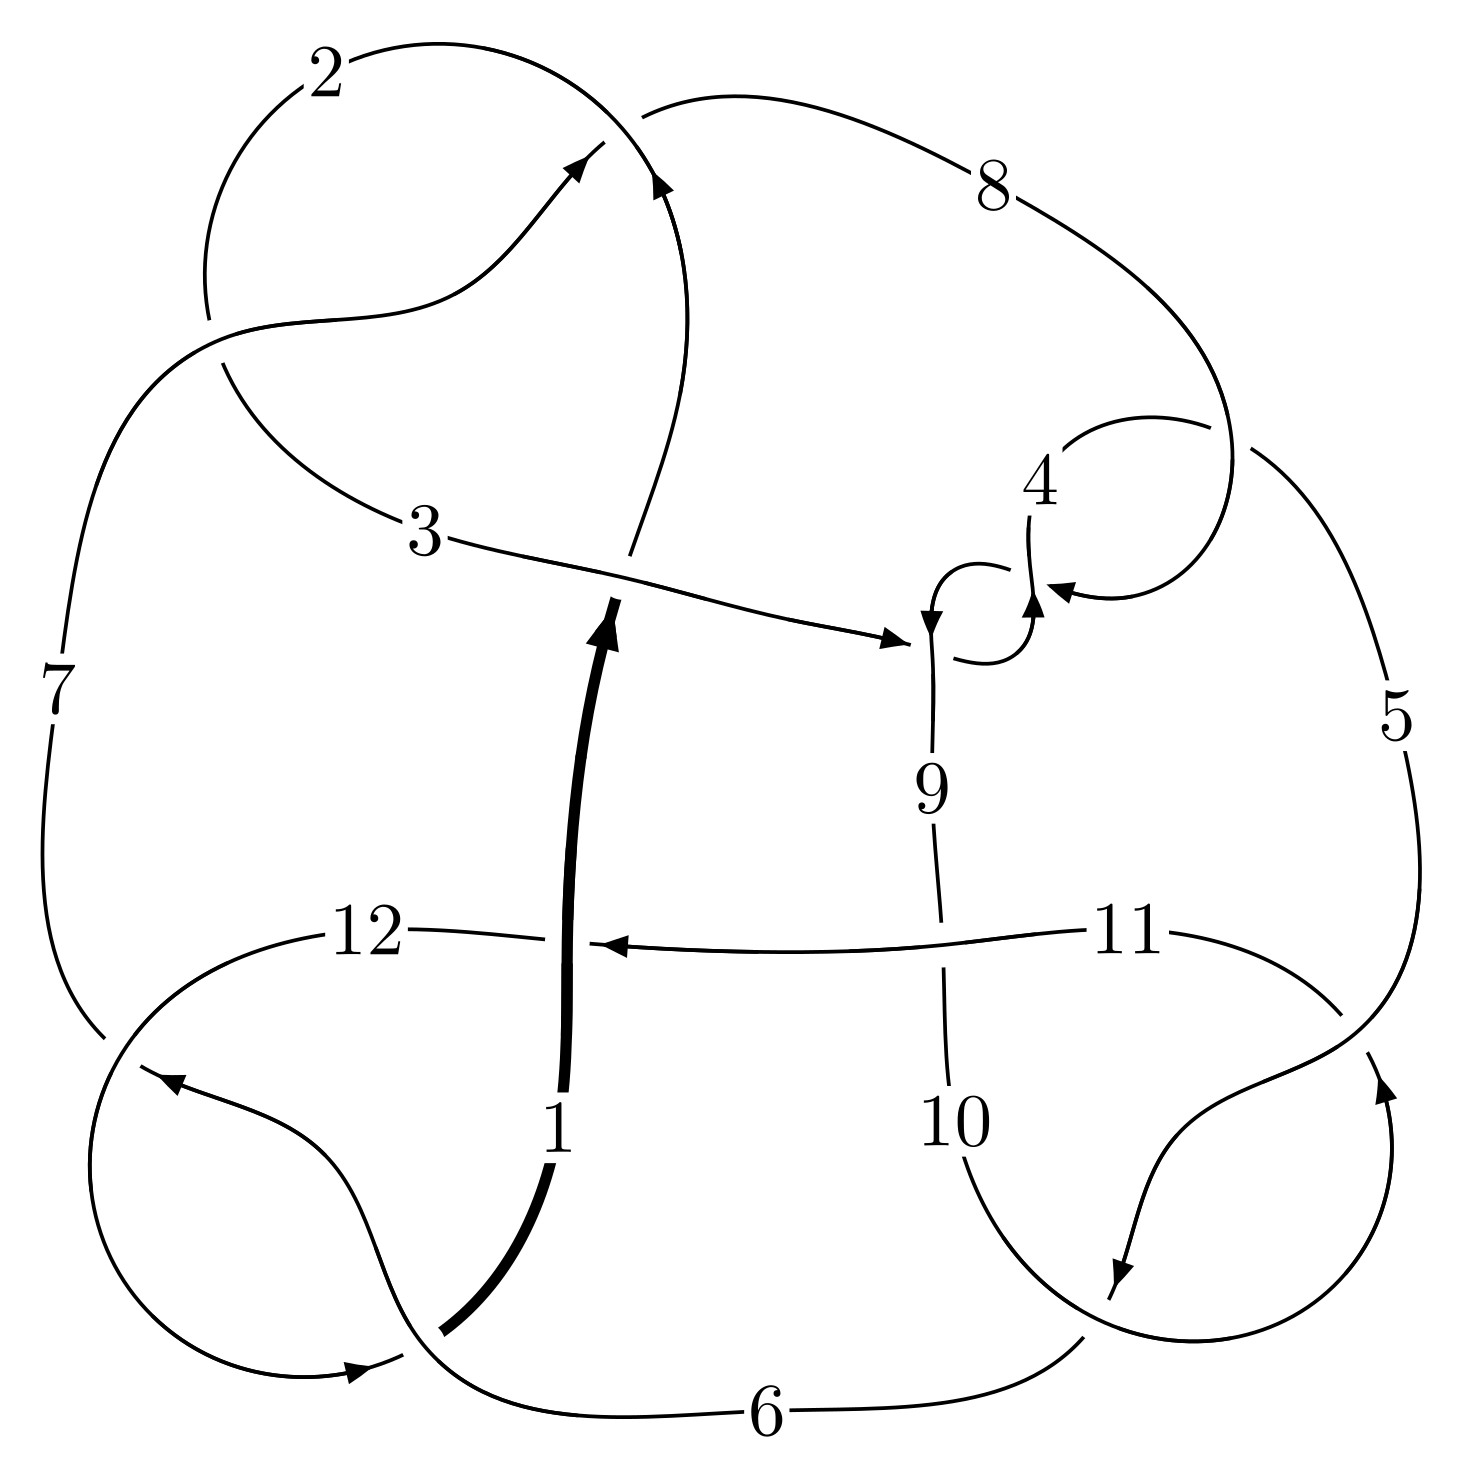
\includegraphics[width=112pt]{../../../GIT/diagram.site/Diagrams/png/1355_12a_0554.png}\\
\ \ \ A knot diagram\footnotemark}&
\allowdisplaybreaks
\textbf{Linearized knot diagam} \\
\cline{2-2}
 &
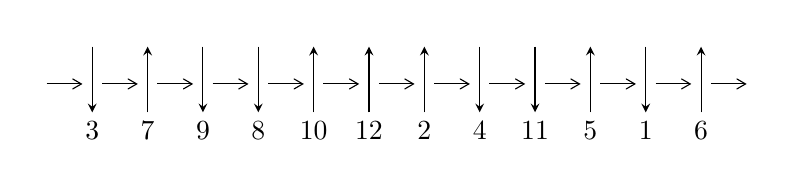
\begin{tikzpicture}[x=20pt, y=17pt]
	% nodes
	\node (C0) at (0, 0) {};
	\node (C1) at (1, 0) {};
	\node (C1U) at (1, +1) {};
	\node (C1D) at (1, -1) {3};

	\node (C2) at (2, 0) {};
	\node (C2U) at (2, +1) {};
	\node (C2D) at (2, -1) {7};

	\node (C3) at (3, 0) {};
	\node (C3U) at (3, +1) {};
	\node (C3D) at (3, -1) {9};

	\node (C4) at (4, 0) {};
	\node (C4U) at (4, +1) {};
	\node (C4D) at (4, -1) {8};

	\node (C5) at (5, 0) {};
	\node (C5U) at (5, +1) {};
	\node (C5D) at (5, -1) {10};

	\node (C6) at (6, 0) {};
	\node (C6U) at (6, +1) {};
	\node (C6D) at (6, -1) {12};

	\node (C7) at (7, 0) {};
	\node (C7U) at (7, +1) {};
	\node (C7D) at (7, -1) {2};

	\node (C8) at (8, 0) {};
	\node (C8U) at (8, +1) {};
	\node (C8D) at (8, -1) {4};

	\node (C9) at (9, 0) {};
	\node (C9U) at (9, +1) {};
	\node (C9D) at (9, -1) {11};

	\node (C10) at (10, 0) {};
	\node (C10U) at (10, +1) {};
	\node (C10D) at (10, -1) {5};

	\node (C11) at (11, 0) {};
	\node (C11U) at (11, +1) {};
	\node (C11D) at (11, -1) {1};

	\node (C12) at (12, 0) {};
	\node (C12U) at (12, +1) {};
	\node (C12D) at (12, -1) {6};
	\node (C13) at (13, 0) {};

	% arrows
	\draw[->,>={angle 60}]
	(C0) edge (C1) (C1) edge (C2) (C2) edge (C3) (C3) edge (C4) (C4) edge (C5) (C5) edge (C6) (C6) edge (C7) (C7) edge (C8) (C8) edge (C9) (C9) edge (C10) (C10) edge (C11) (C11) edge (C12) (C12) edge (C13) ;	\draw[->,>=stealth]
	(C1U) edge (C1D) (C2D) edge (C2U) (C3U) edge (C3D) (C4U) edge (C4D) (C5D) edge (C5U) (C6D) edge (C6U) (C7D) edge (C7U) (C8U) edge (C8D) (C9U) edge (C9D) (C10D) edge (C10U) (C11U) edge (C11D) (C12D) edge (C12U) ;
	\end{tikzpicture} \\
\hhline{~~} \\& 
\textbf{Solving Sequence} \\ \cline{2-2} 
 &
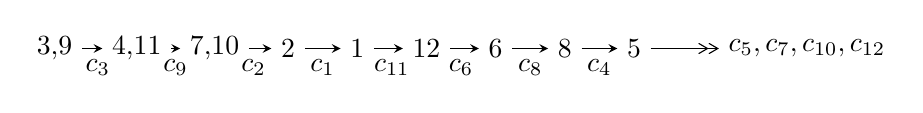
\begin{tikzpicture}[x=25pt, y=7pt]
	% node
	\node (A0) at (-1/8, 0) {3,9};
	\node (A1) at (17/16, 0) {4,11};
	\node (A2) at (35/16, 0) {7,10};
	\node (A3) at (13/4, 0) {2};
	\node (A4) at (17/4, 0) {1};
	\node (A5) at (21/4, 0) {12};
	\node (A6) at (25/4, 0) {6};
	\node (A7) at (29/4, 0) {8};
	\node (A8) at (33/4, 0) {5};
	\node (C1) at (1/2, -1) {$c_{3}$};
	\node (C2) at (13/8, -1) {$c_{9}$};
	\node (C3) at (11/4, -1) {$c_{2}$};
	\node (C4) at (15/4, -1) {$c_{1}$};
	\node (C5) at (19/4, -1) {$c_{11}$};
	\node (C6) at (23/4, -1) {$c_{6}$};
	\node (C7) at (27/4, -1) {$c_{8}$};
	\node (C8) at (31/4, -1) {$c_{4}$};
	\node (A9) at (43/4, 0) {$c_{5},c_{7},c_{10},c_{12}$};

	% edge
	\draw[->,>=stealth]	
	(A0) edge (A1) (A1) edge (A2) (A2) edge (A3) (A3) edge (A4) (A4) edge (A5) (A5) edge (A6) (A6) edge (A7) (A7) edge (A8) ;
	\draw[->>,>={angle 60}]	
	(A8) edge (A9);
\end{tikzpicture} \\ 

\end{tabular} \\

\footnotetext{
The image of knot diagram is generated by the software ``\textbf{Draw programme}" developed by Andrew Bartholomew(\url{http://www.layer8.co.uk/maths/draw/index.htm\#Running-draw}), where we modified some parts for our purpose(\url{https://github.com/CATsTAILs/LinksPainter}).
}\phantom \\ \newline 
\centering \textbf{Ideals for irreducible components\footnotemark of $X_{\text{par}}$} 
 
\begin{align*}
I^u_{1}&=\langle 
- u^{10}+u^9-4 u^8+4 u^7-4 u^6+6 u^5+5 u^3-3 u^2+2 d+2 u-2,\\
\phantom{I^u_{1}}&\phantom{= \langle  }- u^{11}+u^{10}-4 u^9+4 u^8-5 u^7+7 u^6- u^5+7 u^4- u^3+u^2+4 c,\\
\phantom{I^u_{1}}&\phantom{= \langle  }- u^9+u^8-4 u^7+3 u^6-5 u^5+3 u^4-2 u^3+3 u^2+2 b-2 u+2,\\
\phantom{I^u_{1}}&\phantom{= \langle  }- u^{11}- u^{10}-2 u^9-6 u^8+3 u^7-9 u^6+9 u^5- u^4+3 u^3-3 u^2+4 a-4,\\
\phantom{I^u_{1}}&\phantom{= \langle  }u^{12}- u^{11}+6 u^{10}-6 u^9+13 u^8-13 u^7+11 u^6-13 u^5+5 u^4-7 u^3+8 u^2-4 u+4\rangle \\
I^u_{2}&=\langle 
u^4+2 u^2+d,\;- u^9+2 u^8-6 u^7+10 u^6-13 u^5+18 u^4-11 u^3+11 u^2+2 c- u-1,\\
\phantom{I^u_{2}}&\phantom{= \langle  }- u^9-6 u^7+2 u^6-13 u^5+8 u^4-11 u^3+9 u^2+2 b- u+1,\;- u^6-3 u^4-2 u^2+a+1,\\
\phantom{I^u_{2}}&\phantom{= \langle  }u^{10}- u^9+6 u^8-6 u^7+13 u^6-13 u^5+11 u^4-10 u^3+2 u^2+1\rangle \\
I^u_{3}&=\langle 
u^4+2 u^2+d,\;- u^9+2 u^8-6 u^7+10 u^6-13 u^5+18 u^4-11 u^3+11 u^2+2 c- u-1,\\
\phantom{I^u_{3}}&\phantom{= \langle  }u^9+6 u^7-2 u^6+13 u^5-8 u^4+11 u^3-9 u^2+2 b+3 u-1,\\
\phantom{I^u_{3}}&\phantom{= \langle  }3 u^9-4 u^8+20 u^7-22 u^6+49 u^5-46 u^4+49 u^3-37 u^2+2 a+11 u-3,\\
\phantom{I^u_{3}}&\phantom{= \langle  }u^{10}- u^9+6 u^8-6 u^7+13 u^6-13 u^5+11 u^4-10 u^3+2 u^2+1\rangle \\
I^u_{4}&=\langle 
- u^9-4 u^7-3 u^5-2 u^4+7 u^3-5 u^2+2 d+9 u-1,\\
\phantom{I^u_{4}}&\phantom{= \langle  }-3 u^9+2 u^8-18 u^7+14 u^6-39 u^5+34 u^4-33 u^3+29 u^2+2 c-5 u+1,\\
\phantom{I^u_{4}}&\phantom{= \langle  }- u^9-6 u^7+2 u^6-13 u^5+8 u^4-11 u^3+9 u^2+2 b- u+1,\;- u^6-3 u^4-2 u^2+a+1,\\
\phantom{I^u_{4}}&\phantom{= \langle  }u^{10}- u^9+6 u^8-6 u^7+13 u^6-13 u^5+11 u^4-10 u^3+2 u^2+1\rangle \\
I^u_{5}&=\langle 
- u^3+d- u,\;c- u,\;- u^5-2 u^3- u^2+b-1,\;- u^7+2 u^6- u^5+2 u^4+2 u^3+2 a- u+1,\\
\phantom{I^u_{5}}&\phantom{= \langle  }u^8+3 u^6+2 u^5+2 u^4+4 u^3+u^2+u+2\rangle \\
I^u_{6}&=\langle 
u^6+u^5+u^4+3 u^3+d+u+1,\;- u^7- u^5-2 u^4+2 u^3-2 u^2+2 c+u+1,\;b- u,\;a,\\
\phantom{I^u_{6}}&\phantom{= \langle  }u^8+3 u^6+2 u^5+2 u^4+4 u^3+u^2+u+2\rangle \\
I^u_{7}&=\langle 
u^6+u^5+u^4+3 u^3+d+u+1,\;- u^7- u^5-2 u^4+2 u^3-2 u^2+2 c+u+1,\;- u^5-2 u^3- u^2+b-1,\\
\phantom{I^u_{7}}&\phantom{= \langle  }- u^7+2 u^6- u^5+2 u^4+2 u^3+2 a- u+1,\;u^8+3 u^6+2 u^5+2 u^4+4 u^3+u^2+u+2\rangle \\
I^u_{8}&=\langle 
- u^3+d- u,\;c- u,\;b- u,\;a,\;u^4+u^2+u+1\rangle \\
I^u_{9}&=\langle 
u^2+d+u+1,\;c- u,\;- u^2 a- u^2+2 b- a-2,\;2 u^2 a+a^2+4 u^2+2 a+3 u+5,\;u^3+u^2+2 u+1\rangle \\
I^u_{10}&=\langle 
u^2 c+2 c u- u^2+d+c- u-2,\;-2 u^2 c+c^2- c u+3 u^2-4 c+u+5,\;b- u,\;a,\;u^3+u^2+2 u+1\rangle \\
\end{align*}\\
\begin{align*}
I^u_{11}&=\langle 
- u^2 a- a u+2 d- u-3,\;- u^2 a-3 u^2+2 c- a-2 u-6,\;- u^2 a- u^2+2 b- a-2,\\
\phantom{I^u_{11}}&\phantom{= \langle  }2 u^2 a+a^2+4 u^2+2 a+3 u+5,\;u^3+u^2+2 u+1\rangle \\
I^u_{12}&=\langle 
- u^3+d- u,\;c- u,\;b- u,\;a,\;u^6- u^5+2 u^4-2 u^3+2 u^2-2 u+1\rangle \\
I^u_{13}&=\langle 
- u^3+d- u,\;c- u,\;- u^5-2 u^3+u^2+b- u+1,\;u^5- u^4-2 u^2+a,\;u^6- u^5+2 u^4-2 u^3+2 u^2-2 u+1\rangle \\
I^u_{14}&=\langle 
2 u^5- u^4+2 u^3-2 u^2+d+2 u,\;u^4+u^2+c+1,\;b- u,\;a,\;u^6- u^5+2 u^4-2 u^3+2 u^2-2 u+1\rangle \\
I^u_{15}&=\langle 
d+1,\;c- u,\;b,\;a- u,\;u^2+1\rangle \\
I^u_{16}&=\langle 
d+1,\;c- u,\;b- u,\;a-1,\;u^2+1\rangle \\
I^u_{17}&=\langle 
d- u,\;c,\;b- u,\;a-1,\;u^2+1\rangle \\
I^u_{18}&=\langle 
d a+u+1,\;c- u,\;b- u,\;u^2+1\rangle \\
\\
I^v_{1}&=\langle 
a,\;d+v,\;c+a+1,\;b- v,\;v^2+1\rangle \\
\end{align*}
\raggedright * 18 irreducible components of $\dim_{\mathbb{C}}=0$, with total 114 representations.\\
\raggedright * 1 irreducible components of $\dim_{\mathbb{C}}=1$ \\
\footnotetext{All coefficients of polynomials are rational numbers. But the coefficients are sometimes approximated in decimal forms when there is not enough margin.}
\newpage
\renewcommand{\arraystretch}{1}
\centering \section*{I. $I^u_{1}= \langle - u^{10}+u^9+\cdots+2 d-2,\;- u^{11}+u^{10}+\cdots+u^2+4 c,\;- u^9+u^8+\cdots+2 b+2,\;- u^{11}- u^{10}+\cdots+4 a-4,\;u^{12}- u^{11}+\cdots-4 u+4 \rangle$}
\flushleft \textbf{(i) Arc colorings}\\
\begin{tabular}{m{7pt} m{180pt} m{7pt} m{180pt} }
\flushright $a_{3}=$&$\begin{pmatrix}1\\0\end{pmatrix}$ \\
\flushright $a_{9}=$&$\begin{pmatrix}0\\u\end{pmatrix}$ \\
\flushright $a_{4}=$&$\begin{pmatrix}1\\u^2\end{pmatrix}$ \\
\flushright $a_{11}=$&$\begin{pmatrix}\frac{1}{4} u^{11}-\frac{1}{4} u^{10}+\cdots+\frac{1}{4} u^3-\frac{1}{4} u^2\\\frac{1}{2} u^{10}-\frac{1}{2} u^9+\cdots- u+1\end{pmatrix}$ \\
\flushright $a_{7}=$&$\begin{pmatrix}\frac{1}{4} u^{11}+\frac{1}{4} u^{10}+\cdots+\frac{3}{4} u^2+1\\\frac{1}{2} u^9-\frac{1}{2} u^8+\cdots+u-1\end{pmatrix}$ \\
\flushright $a_{10}=$&$\begin{pmatrix}-\frac{1}{4} u^{11}+\frac{1}{4} u^{10}+\cdots- u+1\\-\frac{1}{2} u^9-\frac{5}{2} u^7+\cdots+u+1\end{pmatrix}$ \\
\flushright $a_{2}=$&$\begin{pmatrix}-\frac{1}{4} u^{11}+\frac{3}{4} u^{10}+\cdots-\frac{3}{2} u+1\\-\frac{1}{2} u^{10}+\frac{1}{2} u^9+\cdots+u-1\end{pmatrix}$ \\
\flushright $a_{1}=$&$\begin{pmatrix}-\frac{1}{4} u^{11}+\frac{1}{4} u^{10}+\cdots-\frac{3}{4} u^2-\frac{1}{2} u\\-\frac{1}{2} u^{10}+\frac{1}{2} u^9+\cdots+u-1\end{pmatrix}$ \\
\flushright $a_{12}=$&$\begin{pmatrix}\frac{1}{2} u^{11}-\frac{1}{2} u^{10}+\cdots+\frac{1}{2} u-1\\\frac{1}{2} u^{10}+2 u^8+\cdots+\frac{1}{2} u^2- u\end{pmatrix}$ \\
\flushright $a_{6}=$&$\begin{pmatrix}\frac{1}{4} u^{11}+\frac{1}{4} u^{10}+\cdots-\frac{1}{2} u+1\\-\frac{1}{2} u^{10}+\frac{1}{2} u^9+\cdots+u-1\end{pmatrix}$ \\
\flushright $a_{8}=$&$\begin{pmatrix}u\\u^3+u\end{pmatrix}$ \\
\flushright $a_{5}=$&$\begin{pmatrix}u^2+1\\u^4+2 u^2\end{pmatrix}$\\&\end{tabular}
\flushleft \textbf{(ii) Obstruction class $= -1$}\\~\\
\flushleft \textbf{(iii) Cusp Shapes $= u^{11}+u^{10}+6 u^9+2 u^8+13 u^7- u^6+5 u^5-5 u^4-11 u^3- u^2+2 u+2$}\\~\\
\newpage\renewcommand{\arraystretch}{1}
\flushleft \textbf{(iv) u-Polynomials at the component}\newline \\
\begin{tabular}{m{50pt}|m{274pt}}
Crossings & \hspace{64pt}u-Polynomials at each crossing \\
\hline $$\begin{aligned}c_{1},c_{9},c_{11}\end{aligned}$$&$\begin{aligned}
&u^{12}+5 u^{11}+\cdots+6 u+1
\end{aligned}$\\
\hline $$\begin{aligned}c_{2},c_{5},c_{6}\\c_{7},c_{10},c_{12}\end{aligned}$$&$\begin{aligned}
&u^{12}+u^{11}+3 u^{10}+3 u^9+7 u^8+7 u^7+8 u^6+7 u^5+9 u^4+6 u^3+3 u^2+1
\end{aligned}$\\
\hline $$\begin{aligned}c_{3},c_{4},c_{8}\end{aligned}$$&$\begin{aligned}
&u^{12}+u^{11}+\cdots+4 u+4
\end{aligned}$\\
\hline
\end{tabular}\\~\\
\newpage\renewcommand{\arraystretch}{1}
\flushleft \textbf{(v) Riley Polynomials at the component}\newline \\
\begin{tabular}{m{50pt}|m{274pt}}
Crossings & \hspace{64pt}Riley Polynomials at each crossing \\
\hline $$\begin{aligned}c_{1},c_{9},c_{11}\end{aligned}$$&$\begin{aligned}
&y^{12}+9 y^{11}+\cdots+18 y+1
\end{aligned}$\\
\hline $$\begin{aligned}c_{2},c_{5},c_{6}\\c_{7},c_{10},c_{12}\end{aligned}$$&$\begin{aligned}
&y^{12}+5 y^{11}+\cdots+6 y+1
\end{aligned}$\\
\hline $$\begin{aligned}c_{3},c_{4},c_{8}\end{aligned}$$&$\begin{aligned}
&y^{12}+11 y^{11}+\cdots+48 y+16
\end{aligned}$\\
\hline
\end{tabular}\\~\\
\newpage\flushleft \textbf{(vi) Complex Volumes and Cusp Shapes}
$$\begin{array}{c|c|c}  
\text{Solutions to }I^u_{1}& \I (\text{vol} + \sqrt{-1}CS) & \text{Cusp shape}\\
 \hline 
\begin{aligned}
u &= \phantom{-}0.930547 + 0.179955 I \\
a &= \phantom{-}0.670259 + 1.162990 I \\
b &= -0.563501 + 1.188620 I \\
c &= -1.40294 - 1.16824 I \\
d &= -1.51082 - 1.44889 I\end{aligned}
 & -5.48513 - 12.85560 I & -4.74505 + 9.29863 I \\ \hline\begin{aligned}
u &= \phantom{-}0.930547 - 0.179955 I \\
a &= \phantom{-}0.670259 - 1.162990 I \\
b &= -0.563501 - 1.188620 I \\
c &= -1.40294 + 1.16824 I \\
d &= -1.51082 + 1.44889 I\end{aligned}
 & -5.48513 + 12.85560 I & -4.74505 - 9.29863 I \\ \hline\begin{aligned}
u &= -0.686814 + 0.551480 I \\
a &= -0.796508 + 0.745631 I \\
b &= \phantom{-}0.603454 + 0.816648 I \\
c &= \phantom{-}0.968608 - 0.657314 I \\
d &= -0.163512 - 0.755585 I\end{aligned}
 & \phantom{-}0.72149 + 5.92893 I & \phantom{-}1.32923 - 9.67861 I \\ \hline\begin{aligned}
u &= -0.686814 - 0.551480 I \\
a &= -0.796508 - 0.745631 I \\
b &= \phantom{-}0.603454 - 0.816648 I \\
c &= \phantom{-}0.968608 + 0.657314 I \\
d &= -0.163512 + 0.755585 I\end{aligned}
 & \phantom{-}0.72149 - 5.92893 I & \phantom{-}1.32923 + 9.67861 I \\ \hline\begin{aligned}
u &= \phantom{-}0.185101 + 0.743746 I \\
a &= \phantom{-}0.370768 + 0.449966 I \\
b &= -0.222861 + 0.420471 I \\
c &= -0.277347 + 0.101905 I \\
d &= \phantom{-}0.209277 + 0.422629 I\end{aligned}
 & \phantom{-}0.425064 - 1.127160 I & \phantom{-}4.87896 + 6.40596 I \\ \hline\begin{aligned}
u &= \phantom{-}0.185101 - 0.743746 I \\
a &= \phantom{-}0.370768 - 0.449966 I \\
b &= -0.222861 - 0.420471 I \\
c &= -0.277347 - 0.101905 I \\
d &= \phantom{-}0.209277 - 0.422629 I\end{aligned}
 & \phantom{-}0.425064 + 1.127160 I & \phantom{-}4.87896 - 6.40596 I\\
 \hline 
 \end{array}$$\newpage$$\begin{array}{c|c|c}  
\text{Solutions to }I^u_{1}& \I (\text{vol} + \sqrt{-1}CS) & \text{Cusp shape}\\
 \hline 
\begin{aligned}
u &= -0.18488 + 1.42300 I \\
a &= -1.041110 + 0.719276 I \\
b &= \phantom{-}0.842304 - 0.448362 I \\
c &= -0.567633 - 0.283558 I \\
d &= -0.62794 + 1.29888 I\end{aligned}
 & \phantom{-}7.14373 + 1.01626 I & \phantom{-}7.50962 + 1.51234 I \\ \hline\begin{aligned}
u &= -0.18488 - 1.42300 I \\
a &= -1.041110 - 0.719276 I \\
b &= \phantom{-}0.842304 + 0.448362 I \\
c &= -0.567633 + 0.283558 I \\
d &= -0.62794 - 1.29888 I\end{aligned}
 & \phantom{-}7.14373 - 1.01626 I & \phantom{-}7.50962 - 1.51234 I \\ \hline\begin{aligned}
u &= \phantom{-}0.40234 + 1.40049 I \\
a &= -1.76208 - 0.32910 I \\
b &= \phantom{-}0.593901 - 1.231770 I \\
c &= -1.185730 + 0.490884 I \\
d &= -1.36730 - 2.05780 I\end{aligned}
 & -0.4877 - 17.6327 I & -1.23582 + 10.46043 I \\ \hline\begin{aligned}
u &= \phantom{-}0.40234 - 1.40049 I \\
a &= -1.76208 + 0.32910 I \\
b &= \phantom{-}0.593901 + 1.231770 I \\
c &= -1.185730 - 0.490884 I \\
d &= -1.36730 + 2.05780 I\end{aligned}
 & -0.4877 + 17.6327 I & -1.23582 - 10.46043 I \\ \hline\begin{aligned}
u &= -0.14629 + 1.48775 I \\
a &= \phantom{-}1.55868 + 0.32070 I \\
b &= -0.753298 - 0.941385 I \\
c &= \phantom{-}0.965047 + 0.119356 I \\
d &= \phantom{-}0.460302 - 0.241641 I\end{aligned}
 & \phantom{-}7.55213 + 8.70787 I & \phantom{-}4.26306 - 7.95599 I \\ \hline\begin{aligned}
u &= -0.14629 - 1.48775 I \\
a &= \phantom{-}1.55868 - 0.32070 I \\
b &= -0.753298 + 0.941385 I \\
c &= \phantom{-}0.965047 - 0.119356 I \\
d &= \phantom{-}0.460302 + 0.241641 I\end{aligned}
 & \phantom{-}7.55213 - 8.70787 I & \phantom{-}4.26306 + 7.95599 I\\
 \hline 
 \end{array}$$\newpage\newpage\renewcommand{\arraystretch}{1}
\centering \section*{II. $I^u_{2}= \langle u^4+2 u^2+d,\;- u^9+2 u^8+\cdots+2 c-1,\;- u^9-6 u^7+\cdots+2 b+1,\;- u^6-3 u^4-2 u^2+a+1,\;u^{10}- u^9+\cdots+2 u^2+1 \rangle$}
\flushleft \textbf{(i) Arc colorings}\\
\begin{tabular}{m{7pt} m{180pt} m{7pt} m{180pt} }
\flushright $a_{3}=$&$\begin{pmatrix}1\\0\end{pmatrix}$ \\
\flushright $a_{9}=$&$\begin{pmatrix}0\\u\end{pmatrix}$ \\
\flushright $a_{4}=$&$\begin{pmatrix}1\\u^2\end{pmatrix}$ \\
\flushright $a_{11}=$&$\begin{pmatrix}\frac{1}{2} u^9- u^8+\cdots+\frac{1}{2} u+\frac{1}{2}\\- u^4-2 u^2\end{pmatrix}$ \\
\flushright $a_{7}=$&$\begin{pmatrix}u^6+3 u^4+2 u^2-1\\\frac{1}{2} u^9+3 u^7+\cdots+\frac{1}{2} u-\frac{1}{2}\end{pmatrix}$ \\
\flushright $a_{10}=$&$\begin{pmatrix}-\frac{1}{2} u^9-3 u^7+\cdots+\frac{1}{2} u+\frac{3}{2}\\-\frac{1}{2} u^9-3 u^7+\cdots+\frac{3}{2} u+\frac{1}{2}\end{pmatrix}$ \\
\flushright $a_{2}=$&$\begin{pmatrix}\frac{1}{2} u^9+2 u^7+\cdots-\frac{5}{2} u+\frac{1}{2}\\-\frac{1}{2} u^9-2 u^7+\cdots+\frac{1}{2} u-\frac{1}{2}\end{pmatrix}$ \\
\flushright $a_{1}=$&$\begin{pmatrix}- u^3-2 u\\-\frac{1}{2} u^9-2 u^7+\cdots+\frac{1}{2} u-\frac{1}{2}\end{pmatrix}$ \\
\flushright $a_{12}=$&$\begin{pmatrix}- u^8-5 u^6+u^5-8 u^4+4 u^3-3 u^2+4 u+1\\1\end{pmatrix}$ \\
\flushright $a_{6}=$&$\begin{pmatrix}\frac{1}{2} u^9+2 u^7+\cdots-\frac{5}{2} u+\frac{1}{2}\\- u\end{pmatrix}$ \\
\flushright $a_{8}=$&$\begin{pmatrix}u\\u^3+u\end{pmatrix}$ \\
\flushright $a_{5}=$&$\begin{pmatrix}u^2+1\\u^4+2 u^2\end{pmatrix}$\\&\end{tabular}
\flushleft \textbf{(ii) Obstruction class $= -1$}\\~\\
\flushleft \textbf{(iii) Cusp Shapes $= 4 u^8-2 u^7+20 u^6-10 u^5+32 u^4-20 u^3+12 u^2-14 u-4$}\\~\\
\newpage\renewcommand{\arraystretch}{1}
\flushleft \textbf{(iv) u-Polynomials at the component}\newline \\
\begin{tabular}{m{50pt}|m{274pt}}
Crossings & \hspace{64pt}u-Polynomials at each crossing \\
\hline $$\begin{aligned}c_{1},c_{9}\end{aligned}$$&$\begin{aligned}
&u^{10}+4 u^9+10 u^8+14 u^7+15 u^6+10 u^5+7 u^4+5 u^3+11 u^2+11 u+4
\end{aligned}$\\
\hline $$\begin{aligned}c_{2},c_{5},c_{7}\\c_{10}\end{aligned}$$&$\begin{aligned}
&u^{10}-2 u^9+4 u^8-4 u^7+5 u^6-6 u^5+7 u^4-7 u^3+5 u^2-3 u+2
\end{aligned}$\\
\hline $$\begin{aligned}c_{3},c_{4},c_{8}\end{aligned}$$&$\begin{aligned}
&u^{10}+u^9+6 u^8+6 u^7+13 u^6+13 u^5+11 u^4+10 u^3+2 u^2+1
\end{aligned}$\\
\hline $$\begin{aligned}c_{6},c_{12}\end{aligned}$$&$\begin{aligned}
&u^{10}+u^9+3 u^8+3 u^7+4 u^6+4 u^5+3 u^4+5 u^3+4 u^2+4 u+4
\end{aligned}$\\
\hline $$\begin{aligned}c_{11}\end{aligned}$$&$\begin{aligned}
&u^{10}+5 u^9+11 u^8+13 u^7+8 u^6+2 u^5+u^4- u^3+16 u+16
\end{aligned}$\\
\hline
\end{tabular}\\~\\
\newpage\renewcommand{\arraystretch}{1}
\flushleft \textbf{(v) Riley Polynomials at the component}\newline \\
\begin{tabular}{m{50pt}|m{274pt}}
Crossings & \hspace{64pt}Riley Polynomials at each crossing \\
\hline $$\begin{aligned}c_{1},c_{9}\end{aligned}$$&$\begin{aligned}
&y^{10}+4 y^9+\cdots-33 y+16
\end{aligned}$\\
\hline $$\begin{aligned}c_{2},c_{5},c_{7}\\c_{10}\end{aligned}$$&$\begin{aligned}
&y^{10}+4 y^9+10 y^8+14 y^7+15 y^6+10 y^5+7 y^4+5 y^3+11 y^2+11 y+4
\end{aligned}$\\
\hline $$\begin{aligned}c_{3},c_{4},c_{8}\end{aligned}$$&$\begin{aligned}
&y^{10}+11 y^9+\cdots+4 y+1
\end{aligned}$\\
\hline $$\begin{aligned}c_{6},c_{12}\end{aligned}$$&$\begin{aligned}
&y^{10}+5 y^9+11 y^8+13 y^7+8 y^6+2 y^5+y^4- y^3+16 y+16
\end{aligned}$\\
\hline $$\begin{aligned}c_{11}\end{aligned}$$&$\begin{aligned}
&y^{10}-3 y^9+\cdots-256 y+256
\end{aligned}$\\
\hline
\end{tabular}\\~\\
\newpage\flushleft \textbf{(vi) Complex Volumes and Cusp Shapes}
$$\begin{array}{c|c|c}  
\text{Solutions to }I^u_{2}& \I (\text{vol} + \sqrt{-1}CS) & \text{Cusp shape}\\
 \hline 
\begin{aligned}
u &= \phantom{-}0.748770 + 0.138462 I \\
a &= \phantom{-}0.92253 + 1.26185 I \\
b &= -0.439859 + 1.118370 I \\
c &= -1.60028 - 1.01804 I \\
d &= -1.33318 - 0.63926 I\end{aligned}
 & -7.31978 - 3.81695 I & -7.33347 + 4.73761 I \\ \hline\begin{aligned}
u &= \phantom{-}0.748770 - 0.138462 I \\
a &= \phantom{-}0.92253 - 1.26185 I \\
b &= -0.439859 - 1.118370 I \\
c &= -1.60028 + 1.01804 I \\
d &= -1.33318 + 0.63926 I\end{aligned}
 & -7.31978 + 3.81695 I & -7.33347 - 4.73761 I \\ \hline\begin{aligned}
u &= \phantom{-}0.28433 + 1.41260 I \\
a &= \phantom{-}0.919982 + 0.694170 I \\
b &= -0.910142 - 0.314063 I \\
c &= \phantom{-}0.488875 - 0.418182 I \\
d &= \phantom{-}0.80878 + 1.46934 I\end{aligned}
 & \phantom{-}5.18879 - 6.45670 I & \phantom{-}5.02275 + 3.64794 I \\ \hline\begin{aligned}
u &= \phantom{-}0.28433 - 1.41260 I \\
a &= \phantom{-}0.919982 - 0.694170 I \\
b &= -0.910142 + 0.314063 I \\
c &= \phantom{-}0.488875 + 0.418182 I \\
d &= \phantom{-}0.80878 - 1.46934 I\end{aligned}
 & \phantom{-}5.18879 + 6.45670 I & \phantom{-}5.02275 - 3.64794 I \\ \hline\begin{aligned}
u &= -0.35489 + 1.40814 I \\
a &= \phantom{-}1.79571 - 0.20376 I \\
b &= -0.609606 - 1.180280 I \\
c &= \phantom{-}1.132790 + 0.439888 I \\
d &= \phantom{-}1.26468 - 1.71290 I\end{aligned}
 & \phantom{-}2.57186 + 12.00600 I & \phantom{-}1.91374 - 7.39232 I \\ \hline\begin{aligned}
u &= -0.35489 - 1.40814 I \\
a &= \phantom{-}1.79571 + 0.20376 I \\
b &= -0.609606 + 1.180280 I \\
c &= \phantom{-}1.132790 - 0.439888 I \\
d &= \phantom{-}1.26468 + 1.71290 I\end{aligned}
 & \phantom{-}2.57186 - 12.00600 I & \phantom{-}1.91374 + 7.39232 I\\
 \hline 
 \end{array}$$\newpage$$\begin{array}{c|c|c}  
\text{Solutions to }I^u_{2}& \I (\text{vol} + \sqrt{-1}CS) & \text{Cusp shape}\\
 \hline 
\begin{aligned}
u &= \phantom{-}0.05139 + 1.48296 I \\
a &= -1.43312 + 0.49863 I \\
b &= \phantom{-}0.782018 - 0.812236 I \\
c &= -0.856742 + 0.002799 I \\
d &= -0.408434 + 0.364710 I\end{aligned}
 & \phantom{-}8.34709 - 2.88363 I & \phantom{-}6.09026 + 2.85464 I \\ \hline\begin{aligned}
u &= \phantom{-}0.05139 - 1.48296 I \\
a &= -1.43312 - 0.49863 I \\
b &= \phantom{-}0.782018 + 0.812236 I \\
c &= -0.856742 - 0.002799 I \\
d &= -0.408434 - 0.364710 I\end{aligned}
 & \phantom{-}8.34709 + 2.88363 I & \phantom{-}6.09026 - 2.85464 I \\ \hline\begin{aligned}
u &= -0.229588 + 0.355227 I \\
a &= -1.205100 - 0.252617 I \\
b &= \phantom{-}0.177588 + 0.796469 I \\
c &= \phantom{-}1.33535 + 0.83396 I \\
d &= \phantom{-}0.168159 + 0.302254 I\end{aligned}
 & -3.85316 + 1.05773 I & -3.69328 - 6.23330 I \\ \hline\begin{aligned}
u &= -0.229588 - 0.355227 I \\
a &= -1.205100 + 0.252617 I \\
b &= \phantom{-}0.177588 - 0.796469 I \\
c &= \phantom{-}1.33535 - 0.83396 I \\
d &= \phantom{-}0.168159 - 0.302254 I\end{aligned}
 & -3.85316 - 1.05773 I & -3.69328 + 6.23330 I\\
 \hline 
 \end{array}$$\newpage\newpage\renewcommand{\arraystretch}{1}
\centering \section*{III. $I^u_{3}= \langle u^4+2 u^2+d,\;- u^9+2 u^8+\cdots+2 c-1,\;u^9+6 u^7+\cdots+2 b-1,\;3 u^9-4 u^8+\cdots+2 a-3,\;u^{10}- u^9+\cdots+2 u^2+1 \rangle$}
\flushleft \textbf{(i) Arc colorings}\\
\begin{tabular}{m{7pt} m{180pt} m{7pt} m{180pt} }
\flushright $a_{3}=$&$\begin{pmatrix}1\\0\end{pmatrix}$ \\
\flushright $a_{9}=$&$\begin{pmatrix}0\\u\end{pmatrix}$ \\
\flushright $a_{4}=$&$\begin{pmatrix}1\\u^2\end{pmatrix}$ \\
\flushright $a_{11}=$&$\begin{pmatrix}\frac{1}{2} u^9- u^8+\cdots+\frac{1}{2} u+\frac{1}{2}\\- u^4-2 u^2\end{pmatrix}$ \\
\flushright $a_{7}=$&$\begin{pmatrix}-\frac{3}{2} u^9+2 u^8+\cdots-\frac{11}{2} u+\frac{3}{2}\\-\frac{1}{2} u^9-3 u^7+\cdots-\frac{3}{2} u+\frac{1}{2}\end{pmatrix}$ \\
\flushright $a_{10}=$&$\begin{pmatrix}-\frac{1}{2} u^9-3 u^7+\cdots+\frac{1}{2} u+\frac{3}{2}\\-\frac{1}{2} u^9-3 u^7+\cdots+\frac{3}{2} u+\frac{1}{2}\end{pmatrix}$ \\
\flushright $a_{2}=$&$\begin{pmatrix}- u^9+u^8-5 u^7+5 u^6-9 u^5+8 u^4-5 u^3+2 u^2+2 u-3\\\frac{1}{2} u^9+2 u^7+\cdots-\frac{1}{2} u-\frac{3}{2}\end{pmatrix}$ \\
\flushright $a_{1}=$&$\begin{pmatrix}-\frac{1}{2} u^9+u^8+\cdots+\frac{3}{2} u-\frac{9}{2}\\\frac{1}{2} u^9+2 u^7+\cdots-\frac{1}{2} u-\frac{3}{2}\end{pmatrix}$ \\
\flushright $a_{12}=$&$\begin{pmatrix}u^9- u^8+6 u^7-5 u^6+12 u^5-8 u^4+7 u^3-2 u^2-3 u+3\\1\end{pmatrix}$ \\
\flushright $a_{6}=$&$\begin{pmatrix}\frac{1}{2} u^9+2 u^7+\cdots-\frac{5}{2} u+\frac{1}{2}\\- u\end{pmatrix}$ \\
\flushright $a_{8}=$&$\begin{pmatrix}u\\u^3+u\end{pmatrix}$ \\
\flushright $a_{5}=$&$\begin{pmatrix}u^2+1\\u^4+2 u^2\end{pmatrix}$\\&\end{tabular}
\flushleft \textbf{(ii) Obstruction class $= -1$}\\~\\
\flushleft \textbf{(iii) Cusp Shapes $= 4 u^8-2 u^7+20 u^6-10 u^5+32 u^4-20 u^3+12 u^2-14 u-4$}\\~\\
\newpage\renewcommand{\arraystretch}{1}
\flushleft \textbf{(iv) u-Polynomials at the component}\newline \\
\begin{tabular}{m{50pt}|m{274pt}}
Crossings & \hspace{64pt}u-Polynomials at each crossing \\
\hline $$\begin{aligned}c_{1}\end{aligned}$$&$\begin{aligned}
&u^{10}+5 u^9+11 u^8+13 u^7+8 u^6+2 u^5+u^4- u^3+16 u+16
\end{aligned}$\\
\hline $$\begin{aligned}c_{2},c_{7}\end{aligned}$$&$\begin{aligned}
&u^{10}+u^9+3 u^8+3 u^7+4 u^6+4 u^5+3 u^4+5 u^3+4 u^2+4 u+4
\end{aligned}$\\
\hline $$\begin{aligned}c_{3},c_{4},c_{8}\end{aligned}$$&$\begin{aligned}
&u^{10}+u^9+6 u^8+6 u^7+13 u^6+13 u^5+11 u^4+10 u^3+2 u^2+1
\end{aligned}$\\
\hline $$\begin{aligned}c_{5},c_{6},c_{10}\\c_{12}\end{aligned}$$&$\begin{aligned}
&u^{10}-2 u^9+4 u^8-4 u^7+5 u^6-6 u^5+7 u^4-7 u^3+5 u^2-3 u+2
\end{aligned}$\\
\hline $$\begin{aligned}c_{9},c_{11}\end{aligned}$$&$\begin{aligned}
&u^{10}+4 u^9+10 u^8+14 u^7+15 u^6+10 u^5+7 u^4+5 u^3+11 u^2+11 u+4
\end{aligned}$\\
\hline
\end{tabular}\\~\\
\newpage\renewcommand{\arraystretch}{1}
\flushleft \textbf{(v) Riley Polynomials at the component}\newline \\
\begin{tabular}{m{50pt}|m{274pt}}
Crossings & \hspace{64pt}Riley Polynomials at each crossing \\
\hline $$\begin{aligned}c_{1}\end{aligned}$$&$\begin{aligned}
&y^{10}-3 y^9+\cdots-256 y+256
\end{aligned}$\\
\hline $$\begin{aligned}c_{2},c_{7}\end{aligned}$$&$\begin{aligned}
&y^{10}+5 y^9+11 y^8+13 y^7+8 y^6+2 y^5+y^4- y^3+16 y+16
\end{aligned}$\\
\hline $$\begin{aligned}c_{3},c_{4},c_{8}\end{aligned}$$&$\begin{aligned}
&y^{10}+11 y^9+\cdots+4 y+1
\end{aligned}$\\
\hline $$\begin{aligned}c_{5},c_{6},c_{10}\\c_{12}\end{aligned}$$&$\begin{aligned}
&y^{10}+4 y^9+10 y^8+14 y^7+15 y^6+10 y^5+7 y^4+5 y^3+11 y^2+11 y+4
\end{aligned}$\\
\hline $$\begin{aligned}c_{9},c_{11}\end{aligned}$$&$\begin{aligned}
&y^{10}+4 y^9+\cdots-33 y+16
\end{aligned}$\\
\hline
\end{tabular}\\~\\
\newpage\flushleft \textbf{(vi) Complex Volumes and Cusp Shapes}
$$\begin{array}{c|c|c}  
\text{Solutions to }I^u_{3}& \I (\text{vol} + \sqrt{-1}CS) & \text{Cusp shape}\\
 \hline 
\begin{aligned}
u &= \phantom{-}0.748770 + 0.138462 I \\
a &= \phantom{-}0.68224 - 1.78754 I \\
b &= -0.308911 - 1.256830 I \\
c &= -1.60028 - 1.01804 I \\
d &= -1.33318 - 0.63926 I\end{aligned}
 & -7.31978 - 3.81695 I & -7.33347 + 4.73761 I \\ \hline\begin{aligned}
u &= \phantom{-}0.748770 - 0.138462 I \\
a &= \phantom{-}0.68224 + 1.78754 I \\
b &= -0.308911 + 1.256830 I \\
c &= -1.60028 + 1.01804 I \\
d &= -1.33318 + 0.63926 I\end{aligned}
 & -7.31978 + 3.81695 I & -7.33347 - 4.73761 I \\ \hline\begin{aligned}
u &= \phantom{-}0.28433 + 1.41260 I \\
a &= -1.82670 - 0.00276 I \\
b &= \phantom{-}0.625816 - 1.098530 I \\
c &= \phantom{-}0.488875 - 0.418182 I \\
d &= \phantom{-}0.80878 + 1.46934 I\end{aligned}
 & \phantom{-}5.18879 - 6.45670 I & \phantom{-}5.02275 + 3.64794 I \\ \hline\begin{aligned}
u &= \phantom{-}0.28433 - 1.41260 I \\
a &= -1.82670 + 0.00276 I \\
b &= \phantom{-}0.625816 + 1.098530 I \\
c &= \phantom{-}0.488875 + 0.418182 I \\
d &= \phantom{-}0.80878 - 1.46934 I\end{aligned}
 & \phantom{-}5.18879 + 6.45670 I & \phantom{-}5.02275 - 3.64794 I \\ \hline\begin{aligned}
u &= -0.35489 + 1.40814 I \\
a &= -0.859188 + 0.669926 I \\
b &= \phantom{-}0.964500 - 0.227856 I \\
c &= \phantom{-}1.132790 + 0.439888 I \\
d &= \phantom{-}1.26468 - 1.71290 I\end{aligned}
 & \phantom{-}2.57186 + 12.00600 I & \phantom{-}1.91374 - 7.39232 I \\ \hline\begin{aligned}
u &= -0.35489 - 1.40814 I \\
a &= -0.859188 - 0.669926 I \\
b &= \phantom{-}0.964500 + 0.227856 I \\
c &= \phantom{-}1.132790 - 0.439888 I \\
d &= \phantom{-}1.26468 + 1.71290 I\end{aligned}
 & \phantom{-}2.57186 - 12.00600 I & \phantom{-}1.91374 + 7.39232 I\\
 \hline 
 \end{array}$$\newpage$$\begin{array}{c|c|c}  
\text{Solutions to }I^u_{3}& \I (\text{vol} + \sqrt{-1}CS) & \text{Cusp shape}\\
 \hline 
\begin{aligned}
u &= \phantom{-}0.05139 + 1.48296 I \\
a &= \phantom{-}1.253620 + 0.604304 I \\
b &= -0.833404 - 0.670721 I \\
c &= -0.856742 + 0.002799 I \\
d &= -0.408434 + 0.364710 I\end{aligned}
 & \phantom{-}8.34709 - 2.88363 I & \phantom{-}6.09026 + 2.85464 I \\ \hline\begin{aligned}
u &= \phantom{-}0.05139 - 1.48296 I \\
a &= \phantom{-}1.253620 - 0.604304 I \\
b &= -0.833404 + 0.670721 I \\
c &= -0.856742 - 0.002799 I \\
d &= -0.408434 - 0.364710 I\end{aligned}
 & \phantom{-}8.34709 + 2.88363 I & \phantom{-}6.09026 - 2.85464 I \\ \hline\begin{aligned}
u &= -0.229588 + 0.355227 I \\
a &= -0.74997 - 4.37781 I \\
b &= \phantom{-}0.051999 - 1.151700 I \\
c &= \phantom{-}1.33535 + 0.83396 I \\
d &= \phantom{-}0.168159 + 0.302254 I\end{aligned}
 & -3.85316 + 1.05773 I & -3.69328 - 6.23330 I \\ \hline\begin{aligned}
u &= -0.229588 - 0.355227 I \\
a &= -0.74997 + 4.37781 I \\
b &= \phantom{-}0.051999 + 1.151700 I \\
c &= \phantom{-}1.33535 - 0.83396 I \\
d &= \phantom{-}0.168159 - 0.302254 I\end{aligned}
 & -3.85316 - 1.05773 I & -3.69328 + 6.23330 I\\
 \hline 
 \end{array}$$\newpage\newpage\renewcommand{\arraystretch}{1}
\centering \section*{IV. $I^u_{4}= \langle - u^9-4 u^7+\cdots+2 d-1,\;-3 u^9+2 u^8+\cdots+2 c+1,\;- u^9-6 u^7+\cdots+2 b+1,\;- u^6-3 u^4-2 u^2+a+1,\;u^{10}- u^9+\cdots+2 u^2+1 \rangle$}
\flushleft \textbf{(i) Arc colorings}\\
\begin{tabular}{m{7pt} m{180pt} m{7pt} m{180pt} }
\flushright $a_{3}=$&$\begin{pmatrix}1\\0\end{pmatrix}$ \\
\flushright $a_{9}=$&$\begin{pmatrix}0\\u\end{pmatrix}$ \\
\flushright $a_{4}=$&$\begin{pmatrix}1\\u^2\end{pmatrix}$ \\
\flushright $a_{11}=$&$\begin{pmatrix}\frac{3}{2} u^9- u^8+\cdots+\frac{5}{2} u-\frac{1}{2}\\\frac{1}{2} u^9+2 u^7+\cdots-\frac{9}{2} u+\frac{1}{2}\end{pmatrix}$ \\
\flushright $a_{7}=$&$\begin{pmatrix}u^6+3 u^4+2 u^2-1\\\frac{1}{2} u^9+3 u^7+\cdots+\frac{1}{2} u-\frac{1}{2}\end{pmatrix}$ \\
\flushright $a_{10}=$&$\begin{pmatrix}\frac{5}{2} u^9-2 u^8+\cdots+\frac{7}{2} u-\frac{3}{2}\\u^9+5 u^7+8 u^5+u^3-6 u\end{pmatrix}$ \\
\flushright $a_{2}=$&$\begin{pmatrix}\frac{1}{2} u^9+2 u^7+\cdots-\frac{5}{2} u+\frac{1}{2}\\-\frac{1}{2} u^9-2 u^7+\cdots+\frac{1}{2} u-\frac{1}{2}\end{pmatrix}$ \\
\flushright $a_{1}=$&$\begin{pmatrix}- u^3-2 u\\-\frac{1}{2} u^9-2 u^7+\cdots+\frac{1}{2} u-\frac{1}{2}\end{pmatrix}$ \\
\flushright $a_{12}=$&$\begin{pmatrix}2 u^9- u^8+12 u^7-7 u^6+26 u^5-18 u^4+22 u^3-17 u^2+3 u-1\\u^9+5 u^7+8 u^5+u^3+u^2-6 u\end{pmatrix}$ \\
\flushright $a_{6}=$&$\begin{pmatrix}-\frac{1}{2} u^9-2 u^7+\cdots+\frac{5}{2} u-\frac{7}{2}\\\frac{1}{2} u^9- u^8+\cdots+\frac{3}{2} u+\frac{3}{2}\end{pmatrix}$ \\
\flushright $a_{8}=$&$\begin{pmatrix}u\\u^3+u\end{pmatrix}$ \\
\flushright $a_{5}=$&$\begin{pmatrix}u^2+1\\u^4+2 u^2\end{pmatrix}$\\&\end{tabular}
\flushleft \textbf{(ii) Obstruction class $= -1$}\\~\\
\flushleft \textbf{(iii) Cusp Shapes $= 4 u^8-2 u^7+20 u^6-10 u^5+32 u^4-20 u^3+12 u^2-14 u-4$}\\~\\
\newpage\renewcommand{\arraystretch}{1}
\flushleft \textbf{(iv) u-Polynomials at the component}\newline \\
\begin{tabular}{m{50pt}|m{274pt}}
Crossings & \hspace{64pt}u-Polynomials at each crossing \\
\hline $$\begin{aligned}c_{1},c_{11}\end{aligned}$$&$\begin{aligned}
&u^{10}+4 u^9+10 u^8+14 u^7+15 u^6+10 u^5+7 u^4+5 u^3+11 u^2+11 u+4
\end{aligned}$\\
\hline $$\begin{aligned}c_{2},c_{6},c_{7}\\c_{12}\end{aligned}$$&$\begin{aligned}
&u^{10}-2 u^9+4 u^8-4 u^7+5 u^6-6 u^5+7 u^4-7 u^3+5 u^2-3 u+2
\end{aligned}$\\
\hline $$\begin{aligned}c_{3},c_{4},c_{8}\end{aligned}$$&$\begin{aligned}
&u^{10}+u^9+6 u^8+6 u^7+13 u^6+13 u^5+11 u^4+10 u^3+2 u^2+1
\end{aligned}$\\
\hline $$\begin{aligned}c_{5},c_{10}\end{aligned}$$&$\begin{aligned}
&u^{10}+u^9+3 u^8+3 u^7+4 u^6+4 u^5+3 u^4+5 u^3+4 u^2+4 u+4
\end{aligned}$\\
\hline $$\begin{aligned}c_{9}\end{aligned}$$&$\begin{aligned}
&u^{10}+5 u^9+11 u^8+13 u^7+8 u^6+2 u^5+u^4- u^3+16 u+16
\end{aligned}$\\
\hline
\end{tabular}\\~\\
\newpage\renewcommand{\arraystretch}{1}
\flushleft \textbf{(v) Riley Polynomials at the component}\newline \\
\begin{tabular}{m{50pt}|m{274pt}}
Crossings & \hspace{64pt}Riley Polynomials at each crossing \\
\hline $$\begin{aligned}c_{1},c_{11}\end{aligned}$$&$\begin{aligned}
&y^{10}+4 y^9+\cdots-33 y+16
\end{aligned}$\\
\hline $$\begin{aligned}c_{2},c_{6},c_{7}\\c_{12}\end{aligned}$$&$\begin{aligned}
&y^{10}+4 y^9+10 y^8+14 y^7+15 y^6+10 y^5+7 y^4+5 y^3+11 y^2+11 y+4
\end{aligned}$\\
\hline $$\begin{aligned}c_{3},c_{4},c_{8}\end{aligned}$$&$\begin{aligned}
&y^{10}+11 y^9+\cdots+4 y+1
\end{aligned}$\\
\hline $$\begin{aligned}c_{5},c_{10}\end{aligned}$$&$\begin{aligned}
&y^{10}+5 y^9+11 y^8+13 y^7+8 y^6+2 y^5+y^4- y^3+16 y+16
\end{aligned}$\\
\hline $$\begin{aligned}c_{9}\end{aligned}$$&$\begin{aligned}
&y^{10}-3 y^9+\cdots-256 y+256
\end{aligned}$\\
\hline
\end{tabular}\\~\\
\newpage\flushleft \textbf{(vi) Complex Volumes and Cusp Shapes}
$$\begin{array}{c|c|c}  
\text{Solutions to }I^u_{4}& \I (\text{vol} + \sqrt{-1}CS) & \text{Cusp shape}\\
 \hline 
\begin{aligned}
u &= \phantom{-}0.748770 + 0.138462 I \\
a &= \phantom{-}0.92253 + 1.26185 I \\
b &= -0.439859 + 1.118370 I \\
c &= -1.73122 + 1.35717 I \\
d &= -2.26783 - 0.05446 I\end{aligned}
 & -7.31978 - 3.81695 I & -7.33347 + 4.73761 I \\ \hline\begin{aligned}
u &= \phantom{-}0.748770 - 0.138462 I \\
a &= \phantom{-}0.92253 - 1.26185 I \\
b &= -0.439859 - 1.118370 I \\
c &= -1.73122 - 1.35717 I \\
d &= -2.26783 + 0.05446 I\end{aligned}
 & -7.31978 + 3.81695 I & -7.33347 - 4.73761 I \\ \hline\begin{aligned}
u &= \phantom{-}0.28433 + 1.41260 I \\
a &= \phantom{-}0.919982 + 0.694170 I \\
b &= -0.910142 - 0.314063 I \\
c &= -1.047080 + 0.366289 I \\
d &= -1.16328 - 1.17886 I\end{aligned}
 & \phantom{-}5.18879 - 6.45670 I & \phantom{-}5.02275 + 3.64794 I \\ \hline\begin{aligned}
u &= \phantom{-}0.28433 - 1.41260 I \\
a &= \phantom{-}0.919982 - 0.694170 I \\
b &= -0.910142 + 0.314063 I \\
c &= -1.047080 - 0.366289 I \\
d &= -1.16328 + 1.17886 I\end{aligned}
 & \phantom{-}5.18879 + 6.45670 I & \phantom{-}5.02275 - 3.64794 I \\ \hline\begin{aligned}
u &= -0.35489 + 1.40814 I \\
a &= \phantom{-}1.79571 - 0.20376 I \\
b &= -0.609606 - 1.180280 I \\
c &= -0.441314 - 0.512537 I \\
d &= -0.99330 + 1.55020 I\end{aligned}
 & \phantom{-}2.57186 + 12.00600 I & \phantom{-}1.91374 - 7.39232 I \\ \hline\begin{aligned}
u &= -0.35489 - 1.40814 I \\
a &= \phantom{-}1.79571 + 0.20376 I \\
b &= -0.609606 + 1.180280 I \\
c &= -0.441314 + 0.512537 I \\
d &= -0.99330 - 1.55020 I\end{aligned}
 & \phantom{-}2.57186 - 12.00600 I & \phantom{-}1.91374 + 7.39232 I\\
 \hline 
 \end{array}$$\newpage$$\begin{array}{c|c|c}  
\text{Solutions to }I^u_{4}& \I (\text{vol} + \sqrt{-1}CS) & \text{Cusp shape}\\
 \hline 
\begin{aligned}
u &= \phantom{-}0.05139 + 1.48296 I \\
a &= -1.43312 + 0.49863 I \\
b &= \phantom{-}0.782018 - 0.812236 I \\
c &= \phantom{-}0.758680 - 0.138716 I \\
d &= \phantom{-}0.366987 + 0.885907 I\end{aligned}
 & \phantom{-}8.34709 - 2.88363 I & \phantom{-}6.09026 + 2.85464 I \\ \hline\begin{aligned}
u &= \phantom{-}0.05139 - 1.48296 I \\
a &= -1.43312 - 0.49863 I \\
b &= \phantom{-}0.782018 + 0.812236 I \\
c &= \phantom{-}0.758680 + 0.138716 I \\
d &= \phantom{-}0.366987 - 0.885907 I\end{aligned}
 & \phantom{-}8.34709 + 2.88363 I & \phantom{-}6.09026 - 2.85464 I \\ \hline\begin{aligned}
u &= -0.229588 + 0.355227 I \\
a &= -1.205100 - 0.252617 I \\
b &= \phantom{-}0.177588 + 0.796469 I \\
c &= \phantom{-}1.46094 + 2.78212 I \\
d &= \phantom{-}1.05742 - 2.03840 I\end{aligned}
 & -3.85316 + 1.05773 I & -3.69328 - 6.23330 I \\ \hline\begin{aligned}
u &= -0.229588 - 0.355227 I \\
a &= -1.205100 + 0.252617 I \\
b &= \phantom{-}0.177588 - 0.796469 I \\
c &= \phantom{-}1.46094 - 2.78212 I \\
d &= \phantom{-}1.05742 + 2.03840 I\end{aligned}
 & -3.85316 - 1.05773 I & -3.69328 + 6.23330 I\\
 \hline 
 \end{array}$$\newpage\newpage\renewcommand{\arraystretch}{1}
\centering \section*{V. $I^u_{5}= \langle - u^3+d- u,\;c- u,\;- u^5-2 u^3- u^2+b-1,\;- u^7+2 u^6+\cdots+2 a+1,\;u^8+3 u^6+\cdots+u+2 \rangle$}
\flushleft \textbf{(i) Arc colorings}\\
\begin{tabular}{m{7pt} m{180pt} m{7pt} m{180pt} }
\flushright $a_{3}=$&$\begin{pmatrix}1\\0\end{pmatrix}$ \\
\flushright $a_{9}=$&$\begin{pmatrix}0\\u\end{pmatrix}$ \\
\flushright $a_{4}=$&$\begin{pmatrix}1\\u^2\end{pmatrix}$ \\
\flushright $a_{11}=$&$\begin{pmatrix}u\\u^3+u\end{pmatrix}$ \\
\flushright $a_{7}=$&$\begin{pmatrix}\frac{1}{2} u^7- u^6+\cdots+\frac{1}{2} u-\frac{1}{2}\\u^5+2 u^3+u^2+1\end{pmatrix}$ \\
\flushright $a_{10}=$&$\begin{pmatrix}- u^3\\- u^5- u^3+u\end{pmatrix}$ \\
\flushright $a_{2}=$&$\begin{pmatrix}\frac{1}{2} u^7+u^6+\cdots+\frac{3}{2} u+\frac{1}{2}\\- u^6-2 u^4- u^3- u^2- u-1\end{pmatrix}$ \\
\flushright $a_{1}=$&$\begin{pmatrix}\frac{1}{2} u^7+\frac{1}{2} u^5- u^2+\frac{1}{2} u-\frac{1}{2}\\- u^6-2 u^4- u^3- u^2- u-1\end{pmatrix}$ \\
\flushright $a_{12}=$&$\begin{pmatrix}-\frac{1}{2} u^7+u^6+\cdots+\frac{3}{2} u-\frac{1}{2}\\u^6- u^5+2 u^4+2 u-1\end{pmatrix}$ \\
\flushright $a_{6}=$&$\begin{pmatrix}u^4+u^2+1\\u^6+2 u^4+u^2\end{pmatrix}$ \\
\flushright $a_{8}=$&$\begin{pmatrix}u\\u^3+u\end{pmatrix}$ \\
\flushright $a_{5}=$&$\begin{pmatrix}u^2+1\\u^4+2 u^2\end{pmatrix}$\\&\end{tabular}
\flushleft \textbf{(ii) Obstruction class $= -1$}\\~\\
\flushleft \textbf{(iii) Cusp Shapes $= 4 u^6-4 u^5+8 u^4+8 u+2$}\\~\\
\newpage\renewcommand{\arraystretch}{1}
\flushleft \textbf{(iv) u-Polynomials at the component}\newline \\
\begin{tabular}{m{50pt}|m{274pt}}
Crossings & \hspace{64pt}u-Polynomials at each crossing \\
\hline $$\begin{aligned}c_{1},c_{11}\end{aligned}$$&$\begin{aligned}
&(u^4+2 u^3+3 u^2+u+1)^2
\end{aligned}$\\
\hline $$\begin{aligned}c_{2},c_{6},c_{7}\\c_{12}\end{aligned}$$&$\begin{aligned}
&(u^4+u^2- u+1)^2
\end{aligned}$\\
\hline $$\begin{aligned}c_{3},c_{4},c_{5}\\c_{8},c_{10}\end{aligned}$$&$\begin{aligned}
&u^8+3 u^6-2 u^5+2 u^4-4 u^3+u^2- u+2
\end{aligned}$\\
\hline $$\begin{aligned}c_{9}\end{aligned}$$&$\begin{aligned}
&u^8+6 u^7+13 u^6+10 u^5-2 u^4-4 u^3+u^2+3 u+4
\end{aligned}$\\
\hline
\end{tabular}\\~\\
\newpage\renewcommand{\arraystretch}{1}
\flushleft \textbf{(v) Riley Polynomials at the component}\newline \\
\begin{tabular}{m{50pt}|m{274pt}}
Crossings & \hspace{64pt}Riley Polynomials at each crossing \\
\hline $$\begin{aligned}c_{1},c_{11}\end{aligned}$$&$\begin{aligned}
&(y^4+2 y^3+7 y^2+5 y+1)^2
\end{aligned}$\\
\hline $$\begin{aligned}c_{2},c_{6},c_{7}\\c_{12}\end{aligned}$$&$\begin{aligned}
&(y^4+2 y^3+3 y^2+y+1)^2
\end{aligned}$\\
\hline $$\begin{aligned}c_{3},c_{4},c_{5}\\c_{8},c_{10}\end{aligned}$$&$\begin{aligned}
&y^8+6 y^7+13 y^6+10 y^5-2 y^4-4 y^3+y^2+3 y+4
\end{aligned}$\\
\hline $$\begin{aligned}c_{9}\end{aligned}$$&$\begin{aligned}
&y^8-10 y^7+45 y^6-102 y^5+82 y^4+24 y^3+9 y^2- y+16
\end{aligned}$\\
\hline
\end{tabular}\\~\\
\newpage\flushleft \textbf{(vi) Complex Volumes and Cusp Shapes}
$$\begin{array}{c|c|c}  
\text{Solutions to }I^u_{5}& \I (\text{vol} + \sqrt{-1}CS) & \text{Cusp shape}\\
 \hline 
\begin{aligned}
u &= -0.856926 + 0.228629 I \\
a &= -0.766503 + 1.117310 I \\
b &= \phantom{-}0.547424 + 1.120870 I \\
c &= -0.856926 + 0.228629 I \\
d &= -1.35181 + 0.72034 I\end{aligned}
 & -2.62503 + 7.64338 I & -1.77019 - 6.51087 I \\ \hline\begin{aligned}
u &= -0.856926 - 0.228629 I \\
a &= -0.766503 - 1.117310 I \\
b &= \phantom{-}0.547424 - 1.120870 I \\
c &= -0.856926 - 0.228629 I \\
d &= -1.35181 - 0.72034 I\end{aligned}
 & -2.62503 - 7.64338 I & -1.77019 + 6.51087 I \\ \hline\begin{aligned}
u &= \phantom{-}0.511330 + 0.719091 I \\
a &= \phantom{-}0.699144 + 0.608069 I \\
b &= -0.547424 + 0.585652 I \\
c &= \phantom{-}0.511330 + 0.719091 I \\
d &= -0.148192 + 0.911292 I\end{aligned}
 & \phantom{-}0.98010 - 1.39709 I & \phantom{-}3.77019 + 3.86736 I \\ \hline\begin{aligned}
u &= \phantom{-}0.511330 - 0.719091 I \\
a &= \phantom{-}0.699144 - 0.608069 I \\
b &= -0.547424 - 0.585652 I \\
c &= \phantom{-}0.511330 - 0.719091 I \\
d &= -0.148192 - 0.911292 I\end{aligned}
 & \phantom{-}0.98010 + 1.39709 I & \phantom{-}3.77019 - 3.86736 I \\ \hline\begin{aligned}
u &= \phantom{-}0.036094 + 1.304740 I \\
a &= \phantom{-}1.33473 + 1.08141 I \\
b &= -0.547424 - 0.585652 I \\
c &= \phantom{-}0.036094 + 1.304740 I \\
d &= -0.148192 - 0.911292 I\end{aligned}
 & \phantom{-}0.98010 + 1.39709 I & \phantom{-}3.77019 - 3.86736 I \\ \hline\begin{aligned}
u &= \phantom{-}0.036094 - 1.304740 I \\
a &= \phantom{-}1.33473 - 1.08141 I \\
b &= -0.547424 + 0.585652 I \\
c &= \phantom{-}0.036094 - 1.304740 I \\
d &= -0.148192 + 0.911292 I\end{aligned}
 & \phantom{-}0.98010 - 1.39709 I & \phantom{-}3.77019 + 3.86736 I\\
 \hline 
 \end{array}$$\newpage$$\begin{array}{c|c|c}  
\text{Solutions to }I^u_{5}& \I (\text{vol} + \sqrt{-1}CS) & \text{Cusp shape}\\
 \hline 
\begin{aligned}
u &= \phantom{-}0.309502 + 1.349500 I \\
a &= -2.01737 - 0.12267 I \\
b &= \phantom{-}0.547424 - 1.120870 I \\
c &= \phantom{-}0.309502 + 1.349500 I \\
d &= -1.35181 - 0.72034 I\end{aligned}
 & -2.62503 - 7.64338 I & -1.77019 + 6.51087 I \\ \hline\begin{aligned}
u &= \phantom{-}0.309502 - 1.349500 I \\
a &= -2.01737 + 0.12267 I \\
b &= \phantom{-}0.547424 + 1.120870 I \\
c &= \phantom{-}0.309502 - 1.349500 I \\
d &= -1.35181 + 0.72034 I\end{aligned}
 & -2.62503 + 7.64338 I & -1.77019 - 6.51087 I\\
 \hline 
 \end{array}$$\newpage\newpage\renewcommand{\arraystretch}{1}
\centering \section*{VI. $I^u_{6}= \langle u^6+u^5+\cdots+d+1,\;- u^7- u^5+\cdots+2 c+1,\;b- u,\;a,\;u^8+3 u^6+\cdots+u+2 \rangle$}
\flushleft \textbf{(i) Arc colorings}\\
\begin{tabular}{m{7pt} m{180pt} m{7pt} m{180pt} }
\flushright $a_{3}=$&$\begin{pmatrix}1\\0\end{pmatrix}$ \\
\flushright $a_{9}=$&$\begin{pmatrix}0\\u\end{pmatrix}$ \\
\flushright $a_{4}=$&$\begin{pmatrix}1\\u^2\end{pmatrix}$ \\
\flushright $a_{11}=$&$\begin{pmatrix}\frac{1}{2} u^7+\frac{1}{2} u^5+\cdots-\frac{1}{2} u-\frac{1}{2}\\- u^6- u^5- u^4-3 u^3- u-1\end{pmatrix}$ \\
\flushright $a_{7}=$&$\begin{pmatrix}0\\u\end{pmatrix}$ \\
\flushright $a_{10}=$&$\begin{pmatrix}-\frac{1}{2} u^7-\frac{5}{2} u^5+\cdots-\frac{1}{2} u-\frac{3}{2}\\- u^7-3 u^5-2 u^3- u^2+u-1\end{pmatrix}$ \\
\flushright $a_{2}=$&$\begin{pmatrix}1\\u^2\end{pmatrix}$ \\
\flushright $a_{1}=$&$\begin{pmatrix}u^2+1\\u^2\end{pmatrix}$ \\
\flushright $a_{12}=$&$\begin{pmatrix}\frac{1}{2} u^7+\frac{3}{2} u^5+u^3-\frac{1}{2} u+\frac{1}{2}\\1\end{pmatrix}$ \\
\flushright $a_{6}=$&$\begin{pmatrix}-\frac{1}{2} u^7-\frac{1}{2} u^5+\cdots+\frac{1}{2} u+\frac{1}{2}\\u^5+2 u^3+u^2+u+1\end{pmatrix}$ \\
\flushright $a_{8}=$&$\begin{pmatrix}u\\u^3+u\end{pmatrix}$ \\
\flushright $a_{5}=$&$\begin{pmatrix}u^2+1\\u^4+2 u^2\end{pmatrix}$\\&\end{tabular}
\flushleft \textbf{(ii) Obstruction class $= -1$}\\~\\
\flushleft \textbf{(iii) Cusp Shapes $= 4 u^6-4 u^5+8 u^4+8 u+2$}\\~\\
\newpage\renewcommand{\arraystretch}{1}
\flushleft \textbf{(iv) u-Polynomials at the component}\newline \\
\begin{tabular}{m{50pt}|m{274pt}}
Crossings & \hspace{64pt}u-Polynomials at each crossing \\
\hline $$\begin{aligned}c_{1}\end{aligned}$$&$\begin{aligned}
&u^8+6 u^7+13 u^6+10 u^5-2 u^4-4 u^3+u^2+3 u+4
\end{aligned}$\\
\hline $$\begin{aligned}c_{2},c_{3},c_{4}\\c_{7},c_{8}\end{aligned}$$&$\begin{aligned}
&u^8+3 u^6-2 u^5+2 u^4-4 u^3+u^2- u+2
\end{aligned}$\\
\hline $$\begin{aligned}c_{5},c_{6},c_{10}\\c_{12}\end{aligned}$$&$\begin{aligned}
&(u^4+u^2- u+1)^2
\end{aligned}$\\
\hline $$\begin{aligned}c_{9},c_{11}\end{aligned}$$&$\begin{aligned}
&(u^4+2 u^3+3 u^2+u+1)^2
\end{aligned}$\\
\hline
\end{tabular}\\~\\
\newpage\renewcommand{\arraystretch}{1}
\flushleft \textbf{(v) Riley Polynomials at the component}\newline \\
\begin{tabular}{m{50pt}|m{274pt}}
Crossings & \hspace{64pt}Riley Polynomials at each crossing \\
\hline $$\begin{aligned}c_{1}\end{aligned}$$&$\begin{aligned}
&y^8-10 y^7+45 y^6-102 y^5+82 y^4+24 y^3+9 y^2- y+16
\end{aligned}$\\
\hline $$\begin{aligned}c_{2},c_{3},c_{4}\\c_{7},c_{8}\end{aligned}$$&$\begin{aligned}
&y^8+6 y^7+13 y^6+10 y^5-2 y^4-4 y^3+y^2+3 y+4
\end{aligned}$\\
\hline $$\begin{aligned}c_{5},c_{6},c_{10}\\c_{12}\end{aligned}$$&$\begin{aligned}
&(y^4+2 y^3+3 y^2+y+1)^2
\end{aligned}$\\
\hline $$\begin{aligned}c_{9},c_{11}\end{aligned}$$&$\begin{aligned}
&(y^4+2 y^3+7 y^2+5 y+1)^2
\end{aligned}$\\
\hline
\end{tabular}\\~\\
\newpage\flushleft \textbf{(vi) Complex Volumes and Cusp Shapes}
$$\begin{array}{c|c|c}  
\text{Solutions to }I^u_{6}& \I (\text{vol} + \sqrt{-1}CS) & \text{Cusp shape}\\
 \hline 
\begin{aligned}
u &= -0.856926 + 0.228629 I \\
a &= \phantom{-0.000000 } 0 \\
b &= -0.856926 + 0.228629 I \\
c &= \phantom{-}1.39892 - 1.05885 I \\
d &= \phantom{-}1.17165 - 1.21187 I\end{aligned}
 & -2.62503 + 7.64338 I & -1.77019 - 6.51087 I \\ \hline\begin{aligned}
u &= -0.856926 - 0.228629 I \\
a &= \phantom{-0.000000 } 0 \\
b &= -0.856926 - 0.228629 I \\
c &= \phantom{-}1.39892 + 1.05885 I \\
d &= \phantom{-}1.17165 + 1.21187 I\end{aligned}
 & -2.62503 - 7.64338 I & -1.77019 + 6.51087 I \\ \hline\begin{aligned}
u &= \phantom{-}0.511330 + 0.719091 I \\
a &= \phantom{-0.000000 } 0 \\
b &= \phantom{-}0.511330 + 0.719091 I \\
c &= -0.620678 - 0.381115 I \\
d &= \phantom{-}0.517398 - 0.132058 I\end{aligned}
 & \phantom{-}0.98010 - 1.39709 I & \phantom{-}3.77019 + 3.86736 I \\ \hline\begin{aligned}
u &= \phantom{-}0.511330 - 0.719091 I \\
a &= \phantom{-0.000000 } 0 \\
b &= \phantom{-}0.511330 - 0.719091 I \\
c &= -0.620678 + 0.381115 I \\
d &= \phantom{-}0.517398 + 0.132058 I\end{aligned}
 & \phantom{-}0.98010 + 1.39709 I & \phantom{-}3.77019 - 3.86736 I \\ \hline\begin{aligned}
u &= \phantom{-}0.036094 + 1.304740 I \\
a &= \phantom{-0.000000 } 0 \\
b &= \phantom{-}0.036094 + 1.304740 I \\
c &= \phantom{-}0.490144 + 0.046758 I \\
d &= \phantom{-}0.98671 + 1.09479 I\end{aligned}
 & \phantom{-}0.98010 + 1.39709 I & \phantom{-}3.77019 - 3.86736 I \\ \hline\begin{aligned}
u &= \phantom{-}0.036094 - 1.304740 I \\
a &= \phantom{-0.000000 } 0 \\
b &= \phantom{-}0.036094 - 1.304740 I \\
c &= \phantom{-}0.490144 - 0.046758 I \\
d &= \phantom{-}0.98671 - 1.09479 I\end{aligned}
 & \phantom{-}0.98010 - 1.39709 I & \phantom{-}3.77019 + 3.86736 I\\
 \hline 
 \end{array}$$\newpage$$\begin{array}{c|c|c}  
\text{Solutions to }I^u_{6}& \I (\text{vol} + \sqrt{-1}CS) & \text{Cusp shape}\\
 \hline 
\begin{aligned}
u &= \phantom{-}0.309502 + 1.349500 I \\
a &= \phantom{-0.000000 } 0 \\
b &= \phantom{-}0.309502 + 1.349500 I \\
c &= -1.018380 + 0.475355 I \\
d &= -1.67576 - 1.31818 I\end{aligned}
 & -2.62503 - 7.64338 I & -1.77019 + 6.51087 I \\ \hline\begin{aligned}
u &= \phantom{-}0.309502 - 1.349500 I \\
a &= \phantom{-0.000000 } 0 \\
b &= \phantom{-}0.309502 - 1.349500 I \\
c &= -1.018380 - 0.475355 I \\
d &= -1.67576 + 1.31818 I\end{aligned}
 & -2.62503 + 7.64338 I & -1.77019 - 6.51087 I\\
 \hline 
 \end{array}$$\newpage\newpage\renewcommand{\arraystretch}{1}
\centering \section*{VII. $I^u_{7}= \langle u^6+u^5+\cdots+d+1,\;- u^7- u^5+\cdots+2 c+1,\;- u^5-2 u^3- u^2+b-1,\;- u^7+2 u^6+\cdots+2 a+1,\;u^8+3 u^6+\cdots+u+2 \rangle$}
\flushleft \textbf{(i) Arc colorings}\\
\begin{tabular}{m{7pt} m{180pt} m{7pt} m{180pt} }
\flushright $a_{3}=$&$\begin{pmatrix}1\\0\end{pmatrix}$ \\
\flushright $a_{9}=$&$\begin{pmatrix}0\\u\end{pmatrix}$ \\
\flushright $a_{4}=$&$\begin{pmatrix}1\\u^2\end{pmatrix}$ \\
\flushright $a_{11}=$&$\begin{pmatrix}\frac{1}{2} u^7+\frac{1}{2} u^5+\cdots-\frac{1}{2} u-\frac{1}{2}\\- u^6- u^5- u^4-3 u^3- u-1\end{pmatrix}$ \\
\flushright $a_{7}=$&$\begin{pmatrix}\frac{1}{2} u^7- u^6+\cdots+\frac{1}{2} u-\frac{1}{2}\\u^5+2 u^3+u^2+1\end{pmatrix}$ \\
\flushright $a_{10}=$&$\begin{pmatrix}-\frac{1}{2} u^7-\frac{5}{2} u^5+\cdots-\frac{1}{2} u-\frac{3}{2}\\- u^7-3 u^5-2 u^3- u^2+u-1\end{pmatrix}$ \\
\flushright $a_{2}=$&$\begin{pmatrix}\frac{1}{2} u^7+u^6+\cdots+\frac{3}{2} u+\frac{1}{2}\\- u^6-2 u^4- u^3- u^2- u-1\end{pmatrix}$ \\
\flushright $a_{1}=$&$\begin{pmatrix}\frac{1}{2} u^7+\frac{1}{2} u^5- u^2+\frac{1}{2} u-\frac{1}{2}\\- u^6-2 u^4- u^3- u^2- u-1\end{pmatrix}$ \\
\flushright $a_{12}=$&$\begin{pmatrix}-\frac{1}{2} u^7- u^6+\cdots-\frac{3}{2} u-\frac{1}{2}\\1\end{pmatrix}$ \\
\flushright $a_{6}=$&$\begin{pmatrix}-\frac{1}{2} u^7-\frac{1}{2} u^5+\cdots+\frac{1}{2} u+\frac{1}{2}\\u^5+2 u^3+u^2+u+1\end{pmatrix}$ \\
\flushright $a_{8}=$&$\begin{pmatrix}u\\u^3+u\end{pmatrix}$ \\
\flushright $a_{5}=$&$\begin{pmatrix}u^2+1\\u^4+2 u^2\end{pmatrix}$\\&\end{tabular}
\flushleft \textbf{(ii) Obstruction class $= -1$}\\~\\
\flushleft \textbf{(iii) Cusp Shapes $= 4 u^6-4 u^5+8 u^4+8 u+2$}\\~\\
\newpage\renewcommand{\arraystretch}{1}
\flushleft \textbf{(iv) u-Polynomials at the component}\newline \\
\begin{tabular}{m{50pt}|m{274pt}}
Crossings & \hspace{64pt}u-Polynomials at each crossing \\
\hline $$\begin{aligned}c_{1},c_{9}\end{aligned}$$&$\begin{aligned}
&(u^4+2 u^3+3 u^2+u+1)^2
\end{aligned}$\\
\hline $$\begin{aligned}c_{2},c_{5},c_{7}\\c_{10}\end{aligned}$$&$\begin{aligned}
&(u^4+u^2- u+1)^2
\end{aligned}$\\
\hline $$\begin{aligned}c_{3},c_{4},c_{6}\\c_{8},c_{12}\end{aligned}$$&$\begin{aligned}
&u^8+3 u^6-2 u^5+2 u^4-4 u^3+u^2- u+2
\end{aligned}$\\
\hline $$\begin{aligned}c_{11}\end{aligned}$$&$\begin{aligned}
&u^8+6 u^7+13 u^6+10 u^5-2 u^4-4 u^3+u^2+3 u+4
\end{aligned}$\\
\hline
\end{tabular}\\~\\
\newpage\renewcommand{\arraystretch}{1}
\flushleft \textbf{(v) Riley Polynomials at the component}\newline \\
\begin{tabular}{m{50pt}|m{274pt}}
Crossings & \hspace{64pt}Riley Polynomials at each crossing \\
\hline $$\begin{aligned}c_{1},c_{9}\end{aligned}$$&$\begin{aligned}
&(y^4+2 y^3+7 y^2+5 y+1)^2
\end{aligned}$\\
\hline $$\begin{aligned}c_{2},c_{5},c_{7}\\c_{10}\end{aligned}$$&$\begin{aligned}
&(y^4+2 y^3+3 y^2+y+1)^2
\end{aligned}$\\
\hline $$\begin{aligned}c_{3},c_{4},c_{6}\\c_{8},c_{12}\end{aligned}$$&$\begin{aligned}
&y^8+6 y^7+13 y^6+10 y^5-2 y^4-4 y^3+y^2+3 y+4
\end{aligned}$\\
\hline $$\begin{aligned}c_{11}\end{aligned}$$&$\begin{aligned}
&y^8-10 y^7+45 y^6-102 y^5+82 y^4+24 y^3+9 y^2- y+16
\end{aligned}$\\
\hline
\end{tabular}\\~\\
\newpage\flushleft \textbf{(vi) Complex Volumes and Cusp Shapes}
$$\begin{array}{c|c|c}  
\text{Solutions to }I^u_{7}& \I (\text{vol} + \sqrt{-1}CS) & \text{Cusp shape}\\
 \hline 
\begin{aligned}
u &= -0.856926 + 0.228629 I \\
a &= -0.766503 + 1.117310 I \\
b &= \phantom{-}0.547424 + 1.120870 I \\
c &= \phantom{-}1.39892 - 1.05885 I \\
d &= \phantom{-}1.17165 - 1.21187 I\end{aligned}
 & -2.62503 + 7.64338 I & -1.77019 - 6.51087 I \\ \hline\begin{aligned}
u &= -0.856926 - 0.228629 I \\
a &= -0.766503 - 1.117310 I \\
b &= \phantom{-}0.547424 - 1.120870 I \\
c &= \phantom{-}1.39892 + 1.05885 I \\
d &= \phantom{-}1.17165 + 1.21187 I\end{aligned}
 & -2.62503 - 7.64338 I & -1.77019 + 6.51087 I \\ \hline\begin{aligned}
u &= \phantom{-}0.511330 + 0.719091 I \\
a &= \phantom{-}0.699144 + 0.608069 I \\
b &= -0.547424 + 0.585652 I \\
c &= -0.620678 - 0.381115 I \\
d &= \phantom{-}0.517398 - 0.132058 I\end{aligned}
 & \phantom{-}0.98010 - 1.39709 I & \phantom{-}3.77019 + 3.86736 I \\ \hline\begin{aligned}
u &= \phantom{-}0.511330 - 0.719091 I \\
a &= \phantom{-}0.699144 - 0.608069 I \\
b &= -0.547424 - 0.585652 I \\
c &= -0.620678 + 0.381115 I \\
d &= \phantom{-}0.517398 + 0.132058 I\end{aligned}
 & \phantom{-}0.98010 + 1.39709 I & \phantom{-}3.77019 - 3.86736 I \\ \hline\begin{aligned}
u &= \phantom{-}0.036094 + 1.304740 I \\
a &= \phantom{-}1.33473 + 1.08141 I \\
b &= -0.547424 - 0.585652 I \\
c &= \phantom{-}0.490144 + 0.046758 I \\
d &= \phantom{-}0.98671 + 1.09479 I\end{aligned}
 & \phantom{-}0.98010 + 1.39709 I & \phantom{-}3.77019 - 3.86736 I \\ \hline\begin{aligned}
u &= \phantom{-}0.036094 - 1.304740 I \\
a &= \phantom{-}1.33473 - 1.08141 I \\
b &= -0.547424 + 0.585652 I \\
c &= \phantom{-}0.490144 - 0.046758 I \\
d &= \phantom{-}0.98671 - 1.09479 I\end{aligned}
 & \phantom{-}0.98010 - 1.39709 I & \phantom{-}3.77019 + 3.86736 I\\
 \hline 
 \end{array}$$\newpage$$\begin{array}{c|c|c}  
\text{Solutions to }I^u_{7}& \I (\text{vol} + \sqrt{-1}CS) & \text{Cusp shape}\\
 \hline 
\begin{aligned}
u &= \phantom{-}0.309502 + 1.349500 I \\
a &= -2.01737 - 0.12267 I \\
b &= \phantom{-}0.547424 - 1.120870 I \\
c &= -1.018380 + 0.475355 I \\
d &= -1.67576 - 1.31818 I\end{aligned}
 & -2.62503 - 7.64338 I & -1.77019 + 6.51087 I \\ \hline\begin{aligned}
u &= \phantom{-}0.309502 - 1.349500 I \\
a &= -2.01737 + 0.12267 I \\
b &= \phantom{-}0.547424 + 1.120870 I \\
c &= -1.018380 - 0.475355 I \\
d &= -1.67576 + 1.31818 I\end{aligned}
 & -2.62503 + 7.64338 I & -1.77019 - 6.51087 I\\
 \hline 
 \end{array}$$\newpage\newpage\renewcommand{\arraystretch}{1}
\centering \section*{VIII. $I^u_{8}= \langle - u^3+d- u,\;c- u,\;b- u,\;a,\;u^4+u^2+u+1 \rangle$}
\flushleft \textbf{(i) Arc colorings}\\
\begin{tabular}{m{7pt} m{180pt} m{7pt} m{180pt} }
\flushright $a_{3}=$&$\begin{pmatrix}1\\0\end{pmatrix}$ \\
\flushright $a_{9}=$&$\begin{pmatrix}0\\u\end{pmatrix}$ \\
\flushright $a_{4}=$&$\begin{pmatrix}1\\u^2\end{pmatrix}$ \\
\flushright $a_{11}=$&$\begin{pmatrix}u\\u^3+u\end{pmatrix}$ \\
\flushright $a_{7}=$&$\begin{pmatrix}0\\u\end{pmatrix}$ \\
\flushright $a_{10}=$&$\begin{pmatrix}- u^3\\u^2+2 u\end{pmatrix}$ \\
\flushright $a_{2}=$&$\begin{pmatrix}1\\u^2\end{pmatrix}$ \\
\flushright $a_{1}=$&$\begin{pmatrix}u^2+1\\u^2\end{pmatrix}$ \\
\flushright $a_{12}=$&$\begin{pmatrix}-1\\u^3- u^2-1\end{pmatrix}$ \\
\flushright $a_{6}=$&$\begin{pmatrix}- u\\- u^3- u^2- u-1\end{pmatrix}$ \\
\flushright $a_{8}=$&$\begin{pmatrix}u\\u^3+u\end{pmatrix}$ \\
\flushright $a_{5}=$&$\begin{pmatrix}u^2+1\\u^2- u-1\end{pmatrix}$\\&\end{tabular}
\flushleft \textbf{(ii) Obstruction class $= -1$}\\~\\
\flushleft \textbf{(iii) Cusp Shapes $= 4 u^3-4 u^2+2$}\\~\\
\newpage\renewcommand{\arraystretch}{1}
\flushleft \textbf{(iv) u-Polynomials at the component}\newline \\
\begin{tabular}{m{50pt}|m{274pt}}
Crossings & \hspace{64pt}u-Polynomials at each crossing \\
\hline $$\begin{aligned}c_{1},c_{9},c_{11}\end{aligned}$$&$\begin{aligned}
&u^4+2 u^3+3 u^2+u+1
\end{aligned}$\\
\hline $$\begin{aligned}c_{2},c_{3},c_{4}\\c_{5},c_{6},c_{7}\\c_{8},c_{10},c_{12}\end{aligned}$$&$\begin{aligned}
&u^4+u^2- u+1
\end{aligned}$\\
\hline
\end{tabular}\\~\\
\newpage\renewcommand{\arraystretch}{1}
\flushleft \textbf{(v) Riley Polynomials at the component}\newline \\
\begin{tabular}{m{50pt}|m{274pt}}
Crossings & \hspace{64pt}Riley Polynomials at each crossing \\
\hline $$\begin{aligned}c_{1},c_{9},c_{11}\end{aligned}$$&$\begin{aligned}
&y^4+2 y^3+7 y^2+5 y+1
\end{aligned}$\\
\hline $$\begin{aligned}c_{2},c_{3},c_{4}\\c_{5},c_{6},c_{7}\\c_{8},c_{10},c_{12}\end{aligned}$$&$\begin{aligned}
&y^4+2 y^3+3 y^2+y+1
\end{aligned}$\\
\hline
\end{tabular}\\~\\
\newpage\flushleft \textbf{(vi) Complex Volumes and Cusp Shapes}
$$\begin{array}{c|c|c}  
\text{Solutions to }I^u_{8}& \I (\text{vol} + \sqrt{-1}CS) & \text{Cusp shape}\\
 \hline 
\begin{aligned}
u &= -0.547424 + 0.585652 I \\
a &= \phantom{-0.000000 } 0 \\
b &= -0.547424 + 0.585652 I \\
c &= -0.547424 + 0.585652 I \\
d &= -0.148192 + 0.911292 I\end{aligned}
 & \phantom{-}0.98010 - 1.39709 I & \phantom{-}3.77019 + 3.86736 I \\ \hline\begin{aligned}
u &= -0.547424 - 0.585652 I \\
a &= \phantom{-0.000000 } 0 \\
b &= -0.547424 - 0.585652 I \\
c &= -0.547424 - 0.585652 I \\
d &= -0.148192 - 0.911292 I\end{aligned}
 & \phantom{-}0.98010 + 1.39709 I & \phantom{-}3.77019 - 3.86736 I \\ \hline\begin{aligned}
u &= \phantom{-}0.547424 + 1.120870 I \\
a &= \phantom{-0.000000 } 0 \\
b &= \phantom{-}0.547424 + 1.120870 I \\
c &= \phantom{-}0.547424 + 1.120870 I \\
d &= -1.35181 + 0.72034 I\end{aligned}
 & -2.62503 + 7.64338 I & -1.77019 - 6.51087 I \\ \hline\begin{aligned}
u &= \phantom{-}0.547424 - 1.120870 I \\
a &= \phantom{-0.000000 } 0 \\
b &= \phantom{-}0.547424 - 1.120870 I \\
c &= \phantom{-}0.547424 - 1.120870 I \\
d &= -1.35181 - 0.72034 I\end{aligned}
 & -2.62503 - 7.64338 I & -1.77019 + 6.51087 I\\
 \hline 
 \end{array}$$\newpage\newpage\renewcommand{\arraystretch}{1}
\centering \section*{IX. $I^u_{9}= \langle u^2+d+u+1,\;c- u,\;- u^2 a- u^2+2 b- a-2,\;2 u^2 a+4 u^2+\cdots+2 a+5,\;u^3+u^2+2 u+1 \rangle$}
\flushleft \textbf{(i) Arc colorings}\\
\begin{tabular}{m{7pt} m{180pt} m{7pt} m{180pt} }
\flushright $a_{3}=$&$\begin{pmatrix}1\\0\end{pmatrix}$ \\
\flushright $a_{9}=$&$\begin{pmatrix}0\\u\end{pmatrix}$ \\
\flushright $a_{4}=$&$\begin{pmatrix}1\\u^2\end{pmatrix}$ \\
\flushright $a_{11}=$&$\begin{pmatrix}u\\- u^2- u-1\end{pmatrix}$ \\
\flushright $a_{7}=$&$\begin{pmatrix}a\\\frac{1}{2} u^2 a+\frac{1}{2} u^2+\frac{1}{2} a+1\end{pmatrix}$ \\
\flushright $a_{10}=$&$\begin{pmatrix}u^2+2 u+1\\- u^2\end{pmatrix}$ \\
\flushright $a_{2}=$&$\begin{pmatrix}-\frac{1}{2} u^2 a- a u- u^2- a-\frac{1}{2} u-2\\\frac{1}{2} u^2 a-\frac{1}{2} u^2+\cdots+\frac{1}{2} a-\frac{1}{2}\end{pmatrix}$ \\
\flushright $a_{1}=$&$\begin{pmatrix}-\frac{1}{2} a u-\frac{3}{2} u^2+\cdots-\frac{1}{2} a-\frac{5}{2}\\\frac{1}{2} u^2 a-\frac{1}{2} u^2+\cdots+\frac{1}{2} a-\frac{1}{2}\end{pmatrix}$ \\
\flushright $a_{12}=$&$\begin{pmatrix}\frac{1}{2} u^2 a+3 u^2+a+\frac{5}{2} u+4\\1\end{pmatrix}$ \\
\flushright $a_{6}=$&$\begin{pmatrix}u+2\\- u\end{pmatrix}$ \\
\flushright $a_{8}=$&$\begin{pmatrix}u\\- u^2- u-1\end{pmatrix}$ \\
\flushright $a_{5}=$&$\begin{pmatrix}u^2+1\\u^2+u+1\end{pmatrix}$\\&\end{tabular}
\flushleft \textbf{(ii) Obstruction class $= -1$}\\~\\
\flushleft \textbf{(iii) Cusp Shapes $= -4 u^2-4 u-6$}\\~\\
\newpage\renewcommand{\arraystretch}{1}
\flushleft \textbf{(iv) u-Polynomials at the component}\newline \\
\begin{tabular}{m{50pt}|m{274pt}}
Crossings & \hspace{64pt}u-Polynomials at each crossing \\
\hline $$\begin{aligned}c_{1},c_{11}\end{aligned}$$&$\begin{aligned}
&u^6+3 u^5+4 u^4+2 u^3+1
\end{aligned}$\\
\hline $$\begin{aligned}c_{2},c_{6},c_{7}\\c_{12}\end{aligned}$$&$\begin{aligned}
&u^6+u^5+2 u^4+2 u^3+2 u^2+2 u+1
\end{aligned}$\\
\hline $$\begin{aligned}c_{3},c_{4},c_{5}\\c_{8},c_{10}\end{aligned}$$&$\begin{aligned}
&(u^3- u^2+2 u-1)^2
\end{aligned}$\\
\hline $$\begin{aligned}c_{9}\end{aligned}$$&$\begin{aligned}
&(u^3+3 u^2+2 u-1)^2
\end{aligned}$\\
\hline
\end{tabular}\\~\\
\newpage\renewcommand{\arraystretch}{1}
\flushleft \textbf{(v) Riley Polynomials at the component}\newline \\
\begin{tabular}{m{50pt}|m{274pt}}
Crossings & \hspace{64pt}Riley Polynomials at each crossing \\
\hline $$\begin{aligned}c_{1},c_{11}\end{aligned}$$&$\begin{aligned}
&y^6- y^5+4 y^4-2 y^3+8 y^2+1
\end{aligned}$\\
\hline $$\begin{aligned}c_{2},c_{6},c_{7}\\c_{12}\end{aligned}$$&$\begin{aligned}
&y^6+3 y^5+4 y^4+2 y^3+1
\end{aligned}$\\
\hline $$\begin{aligned}c_{3},c_{4},c_{5}\\c_{8},c_{10}\end{aligned}$$&$\begin{aligned}
&(y^3+3 y^2+2 y-1)^2
\end{aligned}$\\
\hline $$\begin{aligned}c_{9}\end{aligned}$$&$\begin{aligned}
&(y^3-5 y^2+10 y-1)^2
\end{aligned}$\\
\hline
\end{tabular}\\~\\
\newpage\flushleft \textbf{(vi) Complex Volumes and Cusp Shapes}
$$\begin{array}{c|c|c}  
\text{Solutions to }I^u_{9}& \I (\text{vol} + \sqrt{-1}CS) & \text{Cusp shape}\\
 \hline 
\begin{aligned}
u &= -0.215080 + 1.307140 I \\
a &= -0.919774 + 0.855379 I \\
b &= \phantom{-}0.713912 - 0.305839 I \\
c &= -0.215080 + 1.307140 I \\
d &= \phantom{-}0.877439 - 0.744862 I\end{aligned}
 & -0.26574 + 2.82812 I & \phantom{-}1.50976 - 2.97945 I \\ \hline\begin{aligned}
u &= -0.215080 + 1.307140 I \\
a &= \phantom{-}2.24449 + 0.26918 I \\
b &= -0.498832 - 1.001300 I \\
c &= -0.215080 + 1.307140 I \\
d &= \phantom{-}0.877439 - 0.744862 I\end{aligned}
 & -0.26574 + 2.82812 I & \phantom{-}1.50976 - 2.97945 I \\ \hline\begin{aligned}
u &= -0.215080 - 1.307140 I \\
a &= -0.919774 - 0.855379 I \\
b &= \phantom{-}0.713912 + 0.305839 I \\
c &= -0.215080 - 1.307140 I \\
d &= \phantom{-}0.877439 + 0.744862 I\end{aligned}
 & -0.26574 - 2.82812 I & \phantom{-}1.50976 + 2.97945 I \\ \hline\begin{aligned}
u &= -0.215080 - 1.307140 I \\
a &= \phantom{-}2.24449 - 0.26918 I \\
b &= -0.498832 + 1.001300 I \\
c &= -0.215080 - 1.307140 I \\
d &= \phantom{-}0.877439 + 0.744862 I\end{aligned}
 & -0.26574 - 2.82812 I & \phantom{-}1.50976 + 2.97945 I \\ \hline\begin{aligned}
u &= -0.569840\phantom{ +0.000000I} \\
a &= -1.32472 + 1.68359 I \\
b &= \phantom{-}0.284920 + 1.115140 I \\
c &= -0.569840\phantom{ +0.000000I} \\
d &= -0.754878\phantom{ +0.000000I}\end{aligned}
 & -4.40332\phantom{ +0.000000I} & -5.01950\phantom{ +0.000000I} \\ \hline\begin{aligned}
u &= -0.569840\phantom{ +0.000000I} \\
a &= -1.32472 - 1.68359 I \\
b &= \phantom{-}0.284920 - 1.115140 I \\
c &= -0.569840\phantom{ +0.000000I} \\
d &= -0.754878\phantom{ +0.000000I}\end{aligned}
 & -4.40332\phantom{ +0.000000I} & -5.01950\phantom{ +0.000000I}\\
 \hline 
 \end{array}$$\newpage\newpage\renewcommand{\arraystretch}{1}
\centering \section*{X. $I^u_{10}= \langle u^2 c- u^2+\cdots+c-2,\;-2 u^2 c+3 u^2+\cdots-4 c+5,\;b- u,\;a,\;u^3+u^2+2 u+1 \rangle$}
\flushleft \textbf{(i) Arc colorings}\\
\begin{tabular}{m{7pt} m{180pt} m{7pt} m{180pt} }
\flushright $a_{3}=$&$\begin{pmatrix}1\\0\end{pmatrix}$ \\
\flushright $a_{9}=$&$\begin{pmatrix}0\\u\end{pmatrix}$ \\
\flushright $a_{4}=$&$\begin{pmatrix}1\\u^2\end{pmatrix}$ \\
\flushright $a_{11}=$&$\begin{pmatrix}c\\- u^2 c-2 c u+u^2- c+u+2\end{pmatrix}$ \\
\flushright $a_{7}=$&$\begin{pmatrix}0\\u\end{pmatrix}$ \\
\flushright $a_{10}=$&$\begin{pmatrix}u^2 c-2 u^2+2 c- u-3\\- c u\end{pmatrix}$ \\
\flushright $a_{2}=$&$\begin{pmatrix}1\\u^2\end{pmatrix}$ \\
\flushright $a_{1}=$&$\begin{pmatrix}u^2+1\\u^2\end{pmatrix}$ \\
\flushright $a_{12}=$&$\begin{pmatrix}u^2 c+c u-2 u^2+2 c- u-3\\1\end{pmatrix}$ \\
\flushright $a_{6}=$&$\begin{pmatrix}-2 u^2+c- u-4\\- u^2+c-2\end{pmatrix}$ \\
\flushright $a_{8}=$&$\begin{pmatrix}u\\- u^2- u-1\end{pmatrix}$ \\
\flushright $a_{5}=$&$\begin{pmatrix}u^2+1\\u^2+u+1\end{pmatrix}$\\&\end{tabular}
\flushleft \textbf{(ii) Obstruction class $= -1$}\\~\\
\flushleft \textbf{(iii) Cusp Shapes $= -4 u^2-4 u-6$}\\~\\
\newpage\renewcommand{\arraystretch}{1}
\flushleft \textbf{(iv) u-Polynomials at the component}\newline \\
\begin{tabular}{m{50pt}|m{274pt}}
Crossings & \hspace{64pt}u-Polynomials at each crossing \\
\hline $$\begin{aligned}c_{1}\end{aligned}$$&$\begin{aligned}
&(u^3+3 u^2+2 u-1)^2
\end{aligned}$\\
\hline $$\begin{aligned}c_{2},c_{3},c_{4}\\c_{7},c_{8}\end{aligned}$$&$\begin{aligned}
&(u^3- u^2+2 u-1)^2
\end{aligned}$\\
\hline $$\begin{aligned}c_{5},c_{6},c_{10}\\c_{12}\end{aligned}$$&$\begin{aligned}
&u^6+u^5+2 u^4+2 u^3+2 u^2+2 u+1
\end{aligned}$\\
\hline $$\begin{aligned}c_{9},c_{11}\end{aligned}$$&$\begin{aligned}
&u^6+3 u^5+4 u^4+2 u^3+1
\end{aligned}$\\
\hline
\end{tabular}\\~\\
\newpage\renewcommand{\arraystretch}{1}
\flushleft \textbf{(v) Riley Polynomials at the component}\newline \\
\begin{tabular}{m{50pt}|m{274pt}}
Crossings & \hspace{64pt}Riley Polynomials at each crossing \\
\hline $$\begin{aligned}c_{1}\end{aligned}$$&$\begin{aligned}
&(y^3-5 y^2+10 y-1)^2
\end{aligned}$\\
\hline $$\begin{aligned}c_{2},c_{3},c_{4}\\c_{7},c_{8}\end{aligned}$$&$\begin{aligned}
&(y^3+3 y^2+2 y-1)^2
\end{aligned}$\\
\hline $$\begin{aligned}c_{5},c_{6},c_{10}\\c_{12}\end{aligned}$$&$\begin{aligned}
&y^6+3 y^5+4 y^4+2 y^3+1
\end{aligned}$\\
\hline $$\begin{aligned}c_{9},c_{11}\end{aligned}$$&$\begin{aligned}
&y^6- y^5+4 y^4-2 y^3+8 y^2+1
\end{aligned}$\\
\hline
\end{tabular}\\~\\
\newpage\flushleft \textbf{(vi) Complex Volumes and Cusp Shapes}
$$\begin{array}{c|c|c}  
\text{Solutions to }I^u_{10}& \I (\text{vol} + \sqrt{-1}CS) & \text{Cusp shape}\\
 \hline 
\begin{aligned}
u &= -0.215080 + 1.307140 I \\
a &= \phantom{-0.000000 } 0 \\
b &= -0.215080 + 1.307140 I \\
c &= \phantom{-}0.836473 + 0.439023 I \\
d &= \phantom{-}1.93730 - 0.49194 I\end{aligned}
 & -0.26574 + 2.82812 I & \phantom{-}1.50976 - 2.97945 I \\ \hline\begin{aligned}
u &= -0.215080 + 1.307140 I \\
a &= \phantom{-0.000000 } 0 \\
b &= -0.215080 + 1.307140 I \\
c &= -0.376271 - 0.256441 I \\
d &= -0.81474 + 1.23680 I\end{aligned}
 & -0.26574 + 2.82812 I & \phantom{-}1.50976 - 2.97945 I \\ \hline\begin{aligned}
u &= -0.215080 - 1.307140 I \\
a &= \phantom{-0.000000 } 0 \\
b &= -0.215080 - 1.307140 I \\
c &= \phantom{-}0.836473 - 0.439023 I \\
d &= \phantom{-}1.93730 + 0.49194 I\end{aligned}
 & -0.26574 - 2.82812 I & \phantom{-}1.50976 + 2.97945 I \\ \hline\begin{aligned}
u &= -0.215080 - 1.307140 I \\
a &= \phantom{-0.000000 } 0 \\
b &= -0.215080 - 1.307140 I \\
c &= -0.376271 + 0.256441 I \\
d &= -0.81474 - 1.23680 I\end{aligned}
 & -0.26574 - 2.82812 I & \phantom{-}1.50976 + 2.97945 I \\ \hline\begin{aligned}
u &= -0.569840\phantom{ +0.000000I} \\
a &= \phantom{-0.000000 } 0 \\
b &= -0.569840\phantom{ +0.000000I} \\
c &= \phantom{-}2.03980 + 1.11514 I \\
d &= \phantom{-}1.377440 - 0.206343 I\end{aligned}
 & -4.40332\phantom{ +0.000000I} & -5.01950\phantom{ +0.000000I} \\ \hline\begin{aligned}
u &= -0.569840\phantom{ +0.000000I} \\
a &= \phantom{-0.000000 } 0 \\
b &= -0.569840\phantom{ +0.000000I} \\
c &= \phantom{-}2.03980 - 1.11514 I \\
d &= \phantom{-}1.377440 + 0.206343 I\end{aligned}
 & -4.40332\phantom{ +0.000000I} & -5.01950\phantom{ +0.000000I}\\
 \hline 
 \end{array}$$\newpage\newpage\renewcommand{\arraystretch}{1}
\centering \section*{XI. $I^u_{11}= \langle - u^2 a- a u+2 d- u-3,\;- u^2 a-3 u^2+\cdots- a-6,\;- u^2 a- u^2+2 b- a-2,\;2 u^2 a+4 u^2+\cdots+2 a+5,\;u^3+u^2+2 u+1 \rangle$}
\flushleft \textbf{(i) Arc colorings}\\
\begin{tabular}{m{7pt} m{180pt} m{7pt} m{180pt} }
\flushright $a_{3}=$&$\begin{pmatrix}1\\0\end{pmatrix}$ \\
\flushright $a_{9}=$&$\begin{pmatrix}0\\u\end{pmatrix}$ \\
\flushright $a_{4}=$&$\begin{pmatrix}1\\u^2\end{pmatrix}$ \\
\flushright $a_{11}=$&$\begin{pmatrix}\frac{1}{2} u^2 a+\frac{3}{2} u^2+\frac{1}{2} a+u+3\\\frac{1}{2} u^2 a+\frac{1}{2} a u+\frac{1}{2} u+\frac{3}{2}\end{pmatrix}$ \\
\flushright $a_{7}=$&$\begin{pmatrix}a\\\frac{1}{2} u^2 a+\frac{1}{2} u^2+\frac{1}{2} a+1\end{pmatrix}$ \\
\flushright $a_{10}=$&$\begin{pmatrix}u^2 a+\frac{3}{2} u^2+\cdots+\frac{3}{2} a+\frac{7}{2}\\\frac{1}{2} u^2 a+\frac{1}{2} u^2+\cdots+\frac{1}{2} a+\frac{3}{2}\end{pmatrix}$ \\
\flushright $a_{2}=$&$\begin{pmatrix}-\frac{1}{2} u^2 a- a u- u^2- a-\frac{1}{2} u-2\\\frac{1}{2} u^2 a-\frac{1}{2} u^2+\cdots+\frac{1}{2} a-\frac{1}{2}\end{pmatrix}$ \\
\flushright $a_{1}=$&$\begin{pmatrix}-\frac{1}{2} a u-\frac{3}{2} u^2+\cdots-\frac{1}{2} a-\frac{5}{2}\\\frac{1}{2} u^2 a-\frac{1}{2} u^2+\cdots+\frac{1}{2} a-\frac{1}{2}\end{pmatrix}$ \\
\flushright $a_{12}=$&$\begin{pmatrix}\frac{1}{2} u^2 a+a u+u^2+a+\frac{1}{2} u+2\\1\end{pmatrix}$ \\
\flushright $a_{6}=$&$\begin{pmatrix}\frac{1}{2} u^2 a-\frac{1}{2} u^2+\frac{1}{2} a-1\\\frac{1}{2} u^2 a+\frac{1}{2} u^2+\frac{1}{2} a+u+1\end{pmatrix}$ \\
\flushright $a_{8}=$&$\begin{pmatrix}u\\- u^2- u-1\end{pmatrix}$ \\
\flushright $a_{5}=$&$\begin{pmatrix}u^2+1\\u^2+u+1\end{pmatrix}$\\&\end{tabular}
\flushleft \textbf{(ii) Obstruction class $= -1$}\\~\\
\flushleft \textbf{(iii) Cusp Shapes $= -4 u^2-4 u-6$}\\~\\
\newpage\renewcommand{\arraystretch}{1}
\flushleft \textbf{(iv) u-Polynomials at the component}\newline \\
\begin{tabular}{m{50pt}|m{274pt}}
Crossings & \hspace{64pt}u-Polynomials at each crossing \\
\hline $$\begin{aligned}c_{1},c_{9}\end{aligned}$$&$\begin{aligned}
&u^6+3 u^5+4 u^4+2 u^3+1
\end{aligned}$\\
\hline $$\begin{aligned}c_{2},c_{5},c_{7}\\c_{10}\end{aligned}$$&$\begin{aligned}
&u^6+u^5+2 u^4+2 u^3+2 u^2+2 u+1
\end{aligned}$\\
\hline $$\begin{aligned}c_{3},c_{4},c_{6}\\c_{8},c_{12}\end{aligned}$$&$\begin{aligned}
&(u^3- u^2+2 u-1)^2
\end{aligned}$\\
\hline $$\begin{aligned}c_{11}\end{aligned}$$&$\begin{aligned}
&(u^3+3 u^2+2 u-1)^2
\end{aligned}$\\
\hline
\end{tabular}\\~\\
\newpage\renewcommand{\arraystretch}{1}
\flushleft \textbf{(v) Riley Polynomials at the component}\newline \\
\begin{tabular}{m{50pt}|m{274pt}}
Crossings & \hspace{64pt}Riley Polynomials at each crossing \\
\hline $$\begin{aligned}c_{1},c_{9}\end{aligned}$$&$\begin{aligned}
&y^6- y^5+4 y^4-2 y^3+8 y^2+1
\end{aligned}$\\
\hline $$\begin{aligned}c_{2},c_{5},c_{7}\\c_{10}\end{aligned}$$&$\begin{aligned}
&y^6+3 y^5+4 y^4+2 y^3+1
\end{aligned}$\\
\hline $$\begin{aligned}c_{3},c_{4},c_{6}\\c_{8},c_{12}\end{aligned}$$&$\begin{aligned}
&(y^3+3 y^2+2 y-1)^2
\end{aligned}$\\
\hline $$\begin{aligned}c_{11}\end{aligned}$$&$\begin{aligned}
&(y^3-5 y^2+10 y-1)^2
\end{aligned}$\\
\hline
\end{tabular}\\~\\
\newpage\flushleft \textbf{(vi) Complex Volumes and Cusp Shapes}
$$\begin{array}{c|c|c}  
\text{Solutions to }I^u_{11}& \I (\text{vol} + \sqrt{-1}CS) & \text{Cusp shape}\\
 \hline 
\begin{aligned}
u &= -0.215080 + 1.307140 I \\
a &= -0.919774 + 0.855379 I \\
b &= \phantom{-}0.713912 - 0.305839 I \\
c &= \phantom{-}0.836473 + 0.439023 I \\
d &= \phantom{-}1.93730 - 0.49194 I\end{aligned}
 & -0.26574 + 2.82812 I & \phantom{-}1.50976 - 2.97945 I \\ \hline\begin{aligned}
u &= -0.215080 + 1.307140 I \\
a &= \phantom{-}2.24449 + 0.26918 I \\
b &= -0.498832 - 1.001300 I \\
c &= -0.376271 - 0.256441 I \\
d &= -0.81474 + 1.23680 I\end{aligned}
 & -0.26574 + 2.82812 I & \phantom{-}1.50976 - 2.97945 I \\ \hline\begin{aligned}
u &= -0.215080 - 1.307140 I \\
a &= -0.919774 - 0.855379 I \\
b &= \phantom{-}0.713912 + 0.305839 I \\
c &= \phantom{-}0.836473 - 0.439023 I \\
d &= \phantom{-}1.93730 + 0.49194 I\end{aligned}
 & -0.26574 - 2.82812 I & \phantom{-}1.50976 + 2.97945 I \\ \hline\begin{aligned}
u &= -0.215080 - 1.307140 I \\
a &= \phantom{-}2.24449 - 0.26918 I \\
b &= -0.498832 + 1.001300 I \\
c &= -0.376271 + 0.256441 I \\
d &= -0.81474 - 1.23680 I\end{aligned}
 & -0.26574 - 2.82812 I & \phantom{-}1.50976 + 2.97945 I \\ \hline\begin{aligned}
u &= -0.569840\phantom{ +0.000000I} \\
a &= -1.32472 + 1.68359 I \\
b &= \phantom{-}0.284920 + 1.115140 I \\
c &= \phantom{-}2.03980 + 1.11514 I \\
d &= \phantom{-}1.377440 - 0.206343 I\end{aligned}
 & -4.40332\phantom{ +0.000000I} & -5.01950\phantom{ +0.000000I} \\ \hline\begin{aligned}
u &= -0.569840\phantom{ +0.000000I} \\
a &= -1.32472 - 1.68359 I \\
b &= \phantom{-}0.284920 - 1.115140 I \\
c &= \phantom{-}2.03980 - 1.11514 I \\
d &= \phantom{-}1.377440 + 0.206343 I\end{aligned}
 & -4.40332\phantom{ +0.000000I} & -5.01950\phantom{ +0.000000I}\\
 \hline 
 \end{array}$$\newpage\newpage\renewcommand{\arraystretch}{1}
\centering \section*{XII. $I^u_{12}= \langle - u^3+d- u,\;c- u,\;b- u,\;a,\;u^6- u^5+\cdots-2 u+1 \rangle$}
\flushleft \textbf{(i) Arc colorings}\\
\begin{tabular}{m{7pt} m{180pt} m{7pt} m{180pt} }
\flushright $a_{3}=$&$\begin{pmatrix}1\\0\end{pmatrix}$ \\
\flushright $a_{9}=$&$\begin{pmatrix}0\\u\end{pmatrix}$ \\
\flushright $a_{4}=$&$\begin{pmatrix}1\\u^2\end{pmatrix}$ \\
\flushright $a_{11}=$&$\begin{pmatrix}u\\u^3+u\end{pmatrix}$ \\
\flushright $a_{7}=$&$\begin{pmatrix}0\\u\end{pmatrix}$ \\
\flushright $a_{10}=$&$\begin{pmatrix}- u^3\\- u^5- u^3+u\end{pmatrix}$ \\
\flushright $a_{2}=$&$\begin{pmatrix}1\\u^2\end{pmatrix}$ \\
\flushright $a_{1}=$&$\begin{pmatrix}u^2+1\\u^2\end{pmatrix}$ \\
\flushright $a_{12}=$&$\begin{pmatrix}- u^5-2 u^3- u+1\\1\end{pmatrix}$ \\
\flushright $a_{6}=$&$\begin{pmatrix}u^4+u^2+1\\u^5+2 u^3- u^2+2 u-1\end{pmatrix}$ \\
\flushright $a_{8}=$&$\begin{pmatrix}u\\u^3+u\end{pmatrix}$ \\
\flushright $a_{5}=$&$\begin{pmatrix}u^2+1\\u^4+2 u^2\end{pmatrix}$\\&\end{tabular}
\flushleft \textbf{(ii) Obstruction class $= -1$}\\~\\
\flushleft \textbf{(iii) Cusp Shapes $= 4 u^3+4 u-2$}\\~\\
\newpage\renewcommand{\arraystretch}{1}
\flushleft \textbf{(iv) u-Polynomials at the component}\newline \\
\begin{tabular}{m{50pt}|m{274pt}}
Crossings & \hspace{64pt}u-Polynomials at each crossing \\
\hline $$\begin{aligned}c_{1},c_{9},c_{11}\end{aligned}$$&$\begin{aligned}
&u^6+3 u^5+4 u^4+2 u^3+1
\end{aligned}$\\
\hline $$\begin{aligned}c_{2},c_{3},c_{4}\\c_{5},c_{6},c_{7}\\c_{8},c_{10},c_{12}\end{aligned}$$&$\begin{aligned}
&u^6+u^5+2 u^4+2 u^3+2 u^2+2 u+1
\end{aligned}$\\
\hline
\end{tabular}\\~\\
\newpage\renewcommand{\arraystretch}{1}
\flushleft \textbf{(v) Riley Polynomials at the component}\newline \\
\begin{tabular}{m{50pt}|m{274pt}}
Crossings & \hspace{64pt}Riley Polynomials at each crossing \\
\hline $$\begin{aligned}c_{1},c_{9},c_{11}\end{aligned}$$&$\begin{aligned}
&y^6- y^5+4 y^4-2 y^3+8 y^2+1
\end{aligned}$\\
\hline $$\begin{aligned}c_{2},c_{3},c_{4}\\c_{5},c_{6},c_{7}\\c_{8},c_{10},c_{12}\end{aligned}$$&$\begin{aligned}
&y^6+3 y^5+4 y^4+2 y^3+1
\end{aligned}$\\
\hline
\end{tabular}\\~\\
\newpage\flushleft \textbf{(vi) Complex Volumes and Cusp Shapes}
$$\begin{array}{c|c|c}  
\text{Solutions to }I^u_{12}& \I (\text{vol} + \sqrt{-1}CS) & \text{Cusp shape}\\
 \hline 
\begin{aligned}
u &= -0.498832 + 1.001300 I \\
a &= \phantom{-0.000000 } 0 \\
b &= -0.498832 + 1.001300 I \\
c &= -0.498832 + 1.001300 I \\
d &= \phantom{-}0.877439 + 0.744862 I\end{aligned}
 & -0.26574 - 2.82812 I & \phantom{-}1.50976 + 2.97945 I \\ \hline\begin{aligned}
u &= -0.498832 - 1.001300 I \\
a &= \phantom{-0.000000 } 0 \\
b &= -0.498832 - 1.001300 I \\
c &= -0.498832 - 1.001300 I \\
d &= \phantom{-}0.877439 - 0.744862 I\end{aligned}
 & -0.26574 + 2.82812 I & \phantom{-}1.50976 - 2.97945 I \\ \hline\begin{aligned}
u &= \phantom{-}0.284920 + 1.115140 I \\
a &= \phantom{-0.000000 } 0 \\
b &= \phantom{-}0.284920 + 1.115140 I \\
c &= \phantom{-}0.284920 + 1.115140 I \\
d &= -0.754878\phantom{ +0.000000I}\end{aligned}
 & -4.40332\phantom{ +0.000000I} & -5.01951 + 0. I\phantom{ +0.000000I} \\ \hline\begin{aligned}
u &= \phantom{-}0.284920 - 1.115140 I \\
a &= \phantom{-0.000000 } 0 \\
b &= \phantom{-}0.284920 - 1.115140 I \\
c &= \phantom{-}0.284920 - 1.115140 I \\
d &= -0.754878\phantom{ +0.000000I}\end{aligned}
 & -4.40332\phantom{ +0.000000I} & -5.01951 + 0. I\phantom{ +0.000000I} \\ \hline\begin{aligned}
u &= \phantom{-}0.713912 + 0.305839 I \\
a &= \phantom{-0.000000 } 0 \\
b &= \phantom{-}0.713912 + 0.305839 I \\
c &= \phantom{-}0.713912 + 0.305839 I \\
d &= \phantom{-}0.877439 + 0.744862 I\end{aligned}
 & -0.26574 - 2.82812 I & \phantom{-}1.50976 + 2.97945 I \\ \hline\begin{aligned}
u &= \phantom{-}0.713912 - 0.305839 I \\
a &= \phantom{-0.000000 } 0 \\
b &= \phantom{-}0.713912 - 0.305839 I \\
c &= \phantom{-}0.713912 - 0.305839 I \\
d &= \phantom{-}0.877439 - 0.744862 I\end{aligned}
 & -0.26574 + 2.82812 I & \phantom{-}1.50976 - 2.97945 I\\
 \hline 
 \end{array}$$\newpage\newpage\renewcommand{\arraystretch}{1}
\centering \section*{XIII. $I^u_{13}= \langle - u^3+d- u,\;c- u,\;- u^5-2 u^3+\cdots+b+1,\;u^5- u^4-2 u^2+a,\;u^6- u^5+\cdots-2 u+1 \rangle$}
\flushleft \textbf{(i) Arc colorings}\\
\begin{tabular}{m{7pt} m{180pt} m{7pt} m{180pt} }
\flushright $a_{3}=$&$\begin{pmatrix}1\\0\end{pmatrix}$ \\
\flushright $a_{9}=$&$\begin{pmatrix}0\\u\end{pmatrix}$ \\
\flushright $a_{4}=$&$\begin{pmatrix}1\\u^2\end{pmatrix}$ \\
\flushright $a_{11}=$&$\begin{pmatrix}u\\u^3+u\end{pmatrix}$ \\
\flushright $a_{7}=$&$\begin{pmatrix}- u^5+u^4+2 u^2\\u^5+2 u^3- u^2+u-1\end{pmatrix}$ \\
\flushright $a_{10}=$&$\begin{pmatrix}- u^3\\- u^5- u^3+u\end{pmatrix}$ \\
\flushright $a_{2}=$&$\begin{pmatrix}u^5-2 u^4+2 u^3-2 u^2+3 u-2\\- u^5- u^3- u\end{pmatrix}$ \\
\flushright $a_{1}=$&$\begin{pmatrix}-2 u^4+u^3-2 u^2+2 u-2\\- u^5- u^3- u\end{pmatrix}$ \\
\flushright $a_{12}=$&$\begin{pmatrix}- u^5+2 u^4-2 u^3+2 u^2-3 u+2\\1\end{pmatrix}$ \\
\flushright $a_{6}=$&$\begin{pmatrix}u^4+u^2+1\\u^5+2 u^3- u^2+2 u-1\end{pmatrix}$ \\
\flushright $a_{8}=$&$\begin{pmatrix}u\\u^3+u\end{pmatrix}$ \\
\flushright $a_{5}=$&$\begin{pmatrix}u^2+1\\u^4+2 u^2\end{pmatrix}$\\&\end{tabular}
\flushleft \textbf{(ii) Obstruction class $= -1$}\\~\\
\flushleft \textbf{(iii) Cusp Shapes $= 4 u^3+4 u-2$}\\~\\
\newpage\renewcommand{\arraystretch}{1}
\flushleft \textbf{(iv) u-Polynomials at the component}\newline \\
\begin{tabular}{m{50pt}|m{274pt}}
Crossings & \hspace{64pt}u-Polynomials at each crossing \\
\hline $$\begin{aligned}c_{1},c_{9},c_{11}\end{aligned}$$&$\begin{aligned}
&u^6+3 u^5+4 u^4+2 u^3+1
\end{aligned}$\\
\hline $$\begin{aligned}c_{2},c_{3},c_{4}\\c_{5},c_{6},c_{7}\\c_{8},c_{10},c_{12}\end{aligned}$$&$\begin{aligned}
&u^6+u^5+2 u^4+2 u^3+2 u^2+2 u+1
\end{aligned}$\\
\hline
\end{tabular}\\~\\
\newpage\renewcommand{\arraystretch}{1}
\flushleft \textbf{(v) Riley Polynomials at the component}\newline \\
\begin{tabular}{m{50pt}|m{274pt}}
Crossings & \hspace{64pt}Riley Polynomials at each crossing \\
\hline $$\begin{aligned}c_{1},c_{9},c_{11}\end{aligned}$$&$\begin{aligned}
&y^6- y^5+4 y^4-2 y^3+8 y^2+1
\end{aligned}$\\
\hline $$\begin{aligned}c_{2},c_{3},c_{4}\\c_{5},c_{6},c_{7}\\c_{8},c_{10},c_{12}\end{aligned}$$&$\begin{aligned}
&y^6+3 y^5+4 y^4+2 y^3+1
\end{aligned}$\\
\hline
\end{tabular}\\~\\
\newpage\flushleft \textbf{(vi) Complex Volumes and Cusp Shapes}
$$\begin{array}{c|c|c}  
\text{Solutions to }I^u_{13}& \I (\text{vol} + \sqrt{-1}CS) & \text{Cusp shape}\\
 \hline 
\begin{aligned}
u &= -0.498832 + 1.001300 I \\
a &= -0.643729 + 0.689603 I \\
b &= \phantom{-}0.713912 + 0.305839 I \\
c &= -0.498832 + 1.001300 I \\
d &= \phantom{-}0.877439 + 0.744862 I\end{aligned}
 & -0.26574 - 2.82812 I & \phantom{-}1.50976 + 2.97945 I \\ \hline\begin{aligned}
u &= -0.498832 - 1.001300 I \\
a &= -0.643729 - 0.689603 I \\
b &= \phantom{-}0.713912 - 0.305839 I \\
c &= -0.498832 - 1.001300 I \\
d &= \phantom{-}0.877439 - 0.744862 I\end{aligned}
 & -0.26574 + 2.82812 I & \phantom{-}1.50976 - 2.97945 I \\ \hline\begin{aligned}
u &= \phantom{-}0.284920 + 1.115140 I \\
a &= -3.29468 - 0.84179 I \\
b &= \phantom{-}0.284920 - 1.115140 I \\
c &= \phantom{-}0.284920 + 1.115140 I \\
d &= -0.754878\phantom{ +0.000000I}\end{aligned}
 & -4.40332\phantom{ +0.000000I} & -5.01951 + 0. I\phantom{ +0.000000I} \\ \hline\begin{aligned}
u &= \phantom{-}0.284920 - 1.115140 I \\
a &= -3.29468 + 0.84179 I \\
b &= \phantom{-}0.284920 + 1.115140 I \\
c &= \phantom{-}0.284920 - 1.115140 I \\
d &= -0.754878\phantom{ +0.000000I}\end{aligned}
 & -4.40332\phantom{ +0.000000I} & -5.01951 + 0. I\phantom{ +0.000000I} \\ \hline\begin{aligned}
u &= \phantom{-}0.713912 + 0.305839 I \\
a &= \phantom{-}0.938404 + 0.982703 I \\
b &= -0.498832 + 1.001300 I \\
c &= \phantom{-}0.713912 + 0.305839 I \\
d &= \phantom{-}0.877439 + 0.744862 I\end{aligned}
 & -0.26574 - 2.82812 I & \phantom{-}1.50976 + 2.97945 I \\ \hline\begin{aligned}
u &= \phantom{-}0.713912 - 0.305839 I \\
a &= \phantom{-}0.938404 - 0.982703 I \\
b &= -0.498832 - 1.001300 I \\
c &= \phantom{-}0.713912 - 0.305839 I \\
d &= \phantom{-}0.877439 - 0.744862 I\end{aligned}
 & -0.26574 + 2.82812 I & \phantom{-}1.50976 - 2.97945 I\\
 \hline 
 \end{array}$$\newpage\newpage\renewcommand{\arraystretch}{1}
\centering \section*{XIV. $I^u_{14}= \langle 2 u^5- u^4+\cdots+d+2 u,\;u^4+u^2+c+1,\;b- u,\;a,\;u^6- u^5+\cdots-2 u+1 \rangle$}
\flushleft \textbf{(i) Arc colorings}\\
\begin{tabular}{m{7pt} m{180pt} m{7pt} m{180pt} }
\flushright $a_{3}=$&$\begin{pmatrix}1\\0\end{pmatrix}$ \\
\flushright $a_{9}=$&$\begin{pmatrix}0\\u\end{pmatrix}$ \\
\flushright $a_{4}=$&$\begin{pmatrix}1\\u^2\end{pmatrix}$ \\
\flushright $a_{11}=$&$\begin{pmatrix}- u^4- u^2-1\\-2 u^5+u^4-2 u^3+2 u^2-2 u\end{pmatrix}$ \\
\flushright $a_{7}=$&$\begin{pmatrix}0\\u\end{pmatrix}$ \\
\flushright $a_{10}=$&$\begin{pmatrix}-2 u^5-3 u^3+u^2-2 u+1\\-3 u^5+2 u^4-3 u^3+3 u^2-3 u+2\end{pmatrix}$ \\
\flushright $a_{2}=$&$\begin{pmatrix}1\\u^2\end{pmatrix}$ \\
\flushright $a_{1}=$&$\begin{pmatrix}u^2+1\\u^2\end{pmatrix}$ \\
\flushright $a_{12}=$&$\begin{pmatrix}-1\\-2 u^5+2 u^4-2 u^3+2 u^2-2 u\end{pmatrix}$ \\
\flushright $a_{6}=$&$\begin{pmatrix}- u\\2 u^4-2 u^3+2 u^2-3 u+2\end{pmatrix}$ \\
\flushright $a_{8}=$&$\begin{pmatrix}u\\u^3+u\end{pmatrix}$ \\
\flushright $a_{5}=$&$\begin{pmatrix}u^2+1\\u^4+2 u^2\end{pmatrix}$\\&\end{tabular}
\flushleft \textbf{(ii) Obstruction class $= -1$}\\~\\
\flushleft \textbf{(iii) Cusp Shapes $= 4 u^3+4 u-2$}\\~\\
\newpage\renewcommand{\arraystretch}{1}
\flushleft \textbf{(iv) u-Polynomials at the component}\newline \\
\begin{tabular}{m{50pt}|m{274pt}}
Crossings & \hspace{64pt}u-Polynomials at each crossing \\
\hline $$\begin{aligned}c_{1},c_{9},c_{11}\end{aligned}$$&$\begin{aligned}
&u^6+3 u^5+4 u^4+2 u^3+1
\end{aligned}$\\
\hline $$\begin{aligned}c_{2},c_{3},c_{4}\\c_{5},c_{6},c_{7}\\c_{8},c_{10},c_{12}\end{aligned}$$&$\begin{aligned}
&u^6+u^5+2 u^4+2 u^3+2 u^2+2 u+1
\end{aligned}$\\
\hline
\end{tabular}\\~\\
\newpage\renewcommand{\arraystretch}{1}
\flushleft \textbf{(v) Riley Polynomials at the component}\newline \\
\begin{tabular}{m{50pt}|m{274pt}}
Crossings & \hspace{64pt}Riley Polynomials at each crossing \\
\hline $$\begin{aligned}c_{1},c_{9},c_{11}\end{aligned}$$&$\begin{aligned}
&y^6- y^5+4 y^4-2 y^3+8 y^2+1
\end{aligned}$\\
\hline $$\begin{aligned}c_{2},c_{3},c_{4}\\c_{5},c_{6},c_{7}\\c_{8},c_{10},c_{12}\end{aligned}$$&$\begin{aligned}
&y^6+3 y^5+4 y^4+2 y^3+1
\end{aligned}$\\
\hline
\end{tabular}\\~\\
\newpage\flushleft \textbf{(vi) Complex Volumes and Cusp Shapes}
$$\begin{array}{c|c|c}  
\text{Solutions to }I^u_{14}& \I (\text{vol} + \sqrt{-1}CS) & \text{Cusp shape}\\
 \hline 
\begin{aligned}
u &= -0.498832 + 1.001300 I \\
a &= \phantom{-0.000000 } 0 \\
b &= -0.498832 + 1.001300 I \\
c &= \phantom{-}0.183526 - 0.507021 I \\
d &= -1.105040 + 0.381425 I\end{aligned}
 & -0.26574 - 2.82812 I & \phantom{-}1.50976 + 2.97945 I \\ \hline\begin{aligned}
u &= -0.498832 - 1.001300 I \\
a &= \phantom{-0.000000 } 0 \\
b &= -0.498832 - 1.001300 I \\
c &= \phantom{-}0.183526 + 0.507021 I \\
d &= -1.105040 - 0.381425 I\end{aligned}
 & -0.26574 + 2.82812 I & \phantom{-}1.50976 - 2.97945 I \\ \hline\begin{aligned}
u &= \phantom{-}0.284920 + 1.115140 I \\
a &= \phantom{-0.000000 } 0 \\
b &= \phantom{-}0.284920 + 1.115140 I \\
c &= -0.784920 + 0.841795 I \\
d &= -3.70216 - 1.47725 I\end{aligned}
 & -4.40332\phantom{ +0.000000I} & -5.01951 + 0. I\phantom{ +0.000000I} \\ \hline\begin{aligned}
u &= \phantom{-}0.284920 - 1.115140 I \\
a &= \phantom{-0.000000 } 0 \\
b &= \phantom{-}0.284920 - 1.115140 I \\
c &= -0.784920 - 0.841795 I \\
d &= -3.70216 + 1.47725 I\end{aligned}
 & -4.40332\phantom{ +0.000000I} & -5.01951 + 0. I\phantom{ +0.000000I} \\ \hline\begin{aligned}
u &= \phantom{-}0.713912 + 0.305839 I \\
a &= \phantom{-0.000000 } 0 \\
b &= \phantom{-}0.713912 + 0.305839 I \\
c &= -1.39861 - 0.80012 I \\
d &= -0.692808 - 0.761122 I\end{aligned}
 & -0.26574 - 2.82812 I & \phantom{-}1.50976 + 2.97945 I \\ \hline\begin{aligned}
u &= \phantom{-}0.713912 - 0.305839 I \\
a &= \phantom{-0.000000 } 0 \\
b &= \phantom{-}0.713912 - 0.305839 I \\
c &= -1.39861 + 0.80012 I \\
d &= -0.692808 + 0.761122 I\end{aligned}
 & -0.26574 + 2.82812 I & \phantom{-}1.50976 - 2.97945 I\\
 \hline 
 \end{array}$$\newpage\newpage\renewcommand{\arraystretch}{1}
\centering \section*{XV. $I^u_{15}= \langle d+1,\;c- u,\;b,\;a- u,\;u^2+1 \rangle$}
\flushleft \textbf{(i) Arc colorings}\\
\begin{tabular}{m{7pt} m{180pt} m{7pt} m{180pt} }
\flushright $a_{3}=$&$\begin{pmatrix}1\\0\end{pmatrix}$ \\
\flushright $a_{9}=$&$\begin{pmatrix}0\\u\end{pmatrix}$ \\
\flushright $a_{4}=$&$\begin{pmatrix}1\\-1\end{pmatrix}$ \\
\flushright $a_{11}=$&$\begin{pmatrix}u\\-1\end{pmatrix}$ \\
\flushright $a_{7}=$&$\begin{pmatrix}u\\0\end{pmatrix}$ \\
\flushright $a_{10}=$&$\begin{pmatrix}u\\u-1\end{pmatrix}$ \\
\flushright $a_{2}=$&$\begin{pmatrix}1\\0\end{pmatrix}$ \\
\flushright $a_{1}=$&$\begin{pmatrix}1\\0\end{pmatrix}$ \\
\flushright $a_{12}=$&$\begin{pmatrix}u+1\\-1\end{pmatrix}$ \\
\flushright $a_{6}=$&$\begin{pmatrix}1\\u\end{pmatrix}$ \\
\flushright $a_{8}=$&$\begin{pmatrix}u\\0\end{pmatrix}$ \\
\flushright $a_{5}=$&$\begin{pmatrix}0\\-1\end{pmatrix}$\\&\end{tabular}
\flushleft \textbf{(ii) Obstruction class $= 1$}\\~\\
\flushleft \textbf{(iii) Cusp Shapes $= 0$}\\~\\
\newpage\renewcommand{\arraystretch}{1}
\flushleft \textbf{(iv) u-Polynomials at the component}\newline \\
\begin{tabular}{m{50pt}|m{274pt}}
Crossings & \hspace{64pt}u-Polynomials at each crossing \\
\hline $$\begin{aligned}c_{1},c_{2},c_{7}\end{aligned}$$&$\begin{aligned}
&u^2
\end{aligned}$\\
\hline $$\begin{aligned}c_{3},c_{4},c_{5}\\c_{6},c_{8},c_{10}\\c_{12}\end{aligned}$$&$\begin{aligned}
&u^2+1
\end{aligned}$\\
\hline $$\begin{aligned}c_{9},c_{11}\end{aligned}$$&$\begin{aligned}
&(u-1)^2
\end{aligned}$\\
\hline
\end{tabular}\\~\\
\newpage\renewcommand{\arraystretch}{1}
\flushleft \textbf{(v) Riley Polynomials at the component}\newline \\
\begin{tabular}{m{50pt}|m{274pt}}
Crossings & \hspace{64pt}Riley Polynomials at each crossing \\
\hline $$\begin{aligned}c_{1},c_{2},c_{7}\end{aligned}$$&$\begin{aligned}
&y^2
\end{aligned}$\\
\hline $$\begin{aligned}c_{3},c_{4},c_{5}\\c_{6},c_{8},c_{10}\\c_{12}\end{aligned}$$&$\begin{aligned}
&(y+1)^2
\end{aligned}$\\
\hline $$\begin{aligned}c_{9},c_{11}\end{aligned}$$&$\begin{aligned}
&(y-1)^2
\end{aligned}$\\
\hline
\end{tabular}\\~\\
\newpage\flushleft \textbf{(vi) Complex Volumes and Cusp Shapes}
$$\begin{array}{c|c|c}  
\text{Solutions to }I^u_{15}& \I (\text{vol} + \sqrt{-1}CS) & \text{Cusp shape}\\
 \hline 
\begin{aligned}
u &= \phantom{-0.000000 -}1.000000 I \\
a &= \phantom{-0.000000 -}1.000000 I \\
b &= \phantom{-0.000000 } 0 \\
c &= \phantom{-0.000000 -}1.000000 I \\
d &= -1.00000\phantom{ +0.000000I}\end{aligned}
 & -1.64493\phantom{ +0.000000I} & \phantom{-0.000000 } 0 \\ \hline\begin{aligned}
u &= \phantom{-0.000000 } -1.000000 I \\
a &= \phantom{-0.000000 } -1.000000 I \\
b &= \phantom{-0.000000 } 0 \\
c &= \phantom{-0.000000 } -1.000000 I \\
d &= -1.00000\phantom{ +0.000000I}\end{aligned}
 & -1.64493\phantom{ +0.000000I} & \phantom{-0.000000 } 0\\
 \hline 
 \end{array}$$\newpage\newpage\renewcommand{\arraystretch}{1}
\centering \section*{XVI. $I^u_{16}= \langle d+1,\;c- u,\;b- u,\;a-1,\;u^2+1 \rangle$}
\flushleft \textbf{(i) Arc colorings}\\
\begin{tabular}{m{7pt} m{180pt} m{7pt} m{180pt} }
\flushright $a_{3}=$&$\begin{pmatrix}1\\0\end{pmatrix}$ \\
\flushright $a_{9}=$&$\begin{pmatrix}0\\u\end{pmatrix}$ \\
\flushright $a_{4}=$&$\begin{pmatrix}1\\-1\end{pmatrix}$ \\
\flushright $a_{11}=$&$\begin{pmatrix}u\\-1\end{pmatrix}$ \\
\flushright $a_{7}=$&$\begin{pmatrix}1\\u\end{pmatrix}$ \\
\flushright $a_{10}=$&$\begin{pmatrix}u\\u-1\end{pmatrix}$ \\
\flushright $a_{2}=$&$\begin{pmatrix}u+1\\-1\end{pmatrix}$ \\
\flushright $a_{1}=$&$\begin{pmatrix}u\\-1\end{pmatrix}$ \\
\flushright $a_{12}=$&$\begin{pmatrix}u\\-1\end{pmatrix}$ \\
\flushright $a_{6}=$&$\begin{pmatrix}1\\u\end{pmatrix}$ \\
\flushright $a_{8}=$&$\begin{pmatrix}u\\0\end{pmatrix}$ \\
\flushright $a_{5}=$&$\begin{pmatrix}0\\-1\end{pmatrix}$\\&\end{tabular}
\flushleft \textbf{(ii) Obstruction class $= 1$}\\~\\
\flushleft \textbf{(iii) Cusp Shapes $= 0$}\\~\\
\newpage\renewcommand{\arraystretch}{1}
\flushleft \textbf{(iv) u-Polynomials at the component}\newline \\
\begin{tabular}{m{50pt}|m{274pt}}
Crossings & \hspace{64pt}u-Polynomials at each crossing \\
\hline $$\begin{aligned}c_{1},c_{9}\end{aligned}$$&$\begin{aligned}
&(u-1)^2
\end{aligned}$\\
\hline $$\begin{aligned}c_{2},c_{3},c_{4}\\c_{5},c_{7},c_{8}\\c_{10}\end{aligned}$$&$\begin{aligned}
&u^2+1
\end{aligned}$\\
\hline $$\begin{aligned}c_{6},c_{11},c_{12}\end{aligned}$$&$\begin{aligned}
&u^2
\end{aligned}$\\
\hline
\end{tabular}\\~\\
\newpage\renewcommand{\arraystretch}{1}
\flushleft \textbf{(v) Riley Polynomials at the component}\newline \\
\begin{tabular}{m{50pt}|m{274pt}}
Crossings & \hspace{64pt}Riley Polynomials at each crossing \\
\hline $$\begin{aligned}c_{1},c_{9}\end{aligned}$$&$\begin{aligned}
&(y-1)^2
\end{aligned}$\\
\hline $$\begin{aligned}c_{2},c_{3},c_{4}\\c_{5},c_{7},c_{8}\\c_{10}\end{aligned}$$&$\begin{aligned}
&(y+1)^2
\end{aligned}$\\
\hline $$\begin{aligned}c_{6},c_{11},c_{12}\end{aligned}$$&$\begin{aligned}
&y^2
\end{aligned}$\\
\hline
\end{tabular}\\~\\
\newpage\flushleft \textbf{(vi) Complex Volumes and Cusp Shapes}
$$\begin{array}{c|c|c}  
\text{Solutions to }I^u_{16}& \I (\text{vol} + \sqrt{-1}CS) & \text{Cusp shape}\\
 \hline 
\begin{aligned}
u &= \phantom{-0.000000 -}1.000000 I \\
a &= \phantom{-}1.00000\phantom{ +0.000000I} \\
b &= \phantom{-0.000000 -}1.000000 I \\
c &= \phantom{-0.000000 -}1.000000 I \\
d &= -1.00000\phantom{ +0.000000I}\end{aligned}
 & -1.64493\phantom{ +0.000000I} & \phantom{-0.000000 } 0 \\ \hline\begin{aligned}
u &= \phantom{-0.000000 } -1.000000 I \\
a &= \phantom{-}1.00000\phantom{ +0.000000I} \\
b &= \phantom{-0.000000 } -1.000000 I \\
c &= \phantom{-0.000000 } -1.000000 I \\
d &= -1.00000\phantom{ +0.000000I}\end{aligned}
 & -1.64493\phantom{ +0.000000I} & \phantom{-0.000000 } 0\\
 \hline 
 \end{array}$$\newpage\newpage\renewcommand{\arraystretch}{1}
\centering \section*{XVII. $I^u_{17}= \langle d- u,\;c,\;b- u,\;a-1,\;u^2+1 \rangle$}
\flushleft \textbf{(i) Arc colorings}\\
\begin{tabular}{m{7pt} m{180pt} m{7pt} m{180pt} }
\flushright $a_{3}=$&$\begin{pmatrix}1\\0\end{pmatrix}$ \\
\flushright $a_{9}=$&$\begin{pmatrix}0\\u\end{pmatrix}$ \\
\flushright $a_{4}=$&$\begin{pmatrix}1\\-1\end{pmatrix}$ \\
\flushright $a_{11}=$&$\begin{pmatrix}0\\u\end{pmatrix}$ \\
\flushright $a_{7}=$&$\begin{pmatrix}1\\u\end{pmatrix}$ \\
\flushright $a_{10}=$&$\begin{pmatrix}0\\u\end{pmatrix}$ \\
\flushright $a_{2}=$&$\begin{pmatrix}u+1\\-1\end{pmatrix}$ \\
\flushright $a_{1}=$&$\begin{pmatrix}u\\-1\end{pmatrix}$ \\
\flushright $a_{12}=$&$\begin{pmatrix}u\\u-1\end{pmatrix}$ \\
\flushright $a_{6}=$&$\begin{pmatrix}0\\-1\end{pmatrix}$ \\
\flushright $a_{8}=$&$\begin{pmatrix}u\\0\end{pmatrix}$ \\
\flushright $a_{5}=$&$\begin{pmatrix}0\\-1\end{pmatrix}$\\&\end{tabular}
\flushleft \textbf{(ii) Obstruction class $= 1$}\\~\\
\flushleft \textbf{(iii) Cusp Shapes $= 0$}\\~\\
\newpage\renewcommand{\arraystretch}{1}
\flushleft \textbf{(iv) u-Polynomials at the component}\newline \\
\begin{tabular}{m{50pt}|m{274pt}}
Crossings & \hspace{64pt}u-Polynomials at each crossing \\
\hline $$\begin{aligned}c_{1},c_{11}\end{aligned}$$&$\begin{aligned}
&(u-1)^2
\end{aligned}$\\
\hline $$\begin{aligned}c_{2},c_{3},c_{4}\\c_{6},c_{7},c_{8}\\c_{12}\end{aligned}$$&$\begin{aligned}
&u^2+1
\end{aligned}$\\
\hline $$\begin{aligned}c_{5},c_{9},c_{10}\end{aligned}$$&$\begin{aligned}
&u^2
\end{aligned}$\\
\hline
\end{tabular}\\~\\
\newpage\renewcommand{\arraystretch}{1}
\flushleft \textbf{(v) Riley Polynomials at the component}\newline \\
\begin{tabular}{m{50pt}|m{274pt}}
Crossings & \hspace{64pt}Riley Polynomials at each crossing \\
\hline $$\begin{aligned}c_{1},c_{11}\end{aligned}$$&$\begin{aligned}
&(y-1)^2
\end{aligned}$\\
\hline $$\begin{aligned}c_{2},c_{3},c_{4}\\c_{6},c_{7},c_{8}\\c_{12}\end{aligned}$$&$\begin{aligned}
&(y+1)^2
\end{aligned}$\\
\hline $$\begin{aligned}c_{5},c_{9},c_{10}\end{aligned}$$&$\begin{aligned}
&y^2
\end{aligned}$\\
\hline
\end{tabular}\\~\\
\newpage\flushleft \textbf{(vi) Complex Volumes and Cusp Shapes}
$$\begin{array}{c|c|c}  
\text{Solutions to }I^u_{17}& \I (\text{vol} + \sqrt{-1}CS) & \text{Cusp shape}\\
 \hline 
\begin{aligned}
u &= \phantom{-0.000000 -}1.000000 I \\
a &= \phantom{-}1.00000\phantom{ +0.000000I} \\
b &= \phantom{-0.000000 -}1.000000 I \\
c &= \phantom{-0.000000 } 0 \\
d &= \phantom{-0.000000 -}1.000000 I\end{aligned}
 & -1.64493\phantom{ +0.000000I} & \phantom{-0.000000 } 0 \\ \hline\begin{aligned}
u &= \phantom{-0.000000 } -1.000000 I \\
a &= \phantom{-}1.00000\phantom{ +0.000000I} \\
b &= \phantom{-0.000000 } -1.000000 I \\
c &= \phantom{-0.000000 } 0 \\
d &= \phantom{-0.000000 } -1.000000 I\end{aligned}
 & -1.64493\phantom{ +0.000000I} & \phantom{-0.000000 } 0\\
 \hline 
 \end{array}$$\newpage\newpage\renewcommand{\arraystretch}{1}
\centering \section*{XVIII. $I^u_{18}= \langle d a+u+1,\;c- u,\;b- u,\;u^2+1 \rangle$}
\flushleft \textbf{(i) Arc colorings}\\
\begin{tabular}{m{7pt} m{180pt} m{7pt} m{180pt} }
\flushright $a_{3}=$&$\begin{pmatrix}1\\0\end{pmatrix}$ \\
\flushright $a_{9}=$&$\begin{pmatrix}0\\u\end{pmatrix}$ \\
\flushright $a_{4}=$&$\begin{pmatrix}1\\-1\end{pmatrix}$ \\
\flushright $a_{11}=$&$\begin{pmatrix}u\\d\end{pmatrix}$ \\
\flushright $a_{7}=$&$\begin{pmatrix}a\\u\end{pmatrix}$ \\
\flushright $a_{10}=$&$\begin{pmatrix}u\\d+u\end{pmatrix}$ \\
\flushright $a_{2}=$&$\begin{pmatrix}a u+1\\-1\end{pmatrix}$ \\
\flushright $a_{1}=$&$\begin{pmatrix}a u\\-1\end{pmatrix}$ \\
\flushright $a_{12}=$&$\begin{pmatrix}- a u+u\\d+1\end{pmatrix}$ \\
\flushright $a_{6}=$&$\begin{pmatrix}1\\- d u\end{pmatrix}$ \\
\flushright $a_{8}=$&$\begin{pmatrix}u\\0\end{pmatrix}$ \\
\flushright $a_{5}=$&$\begin{pmatrix}0\\-1\end{pmatrix}$\\&\end{tabular}
\flushleft \textbf{(ii) Obstruction class $= -1$}\\~\\
\flushleft \textbf{(iii) Cusp Shapes $= -6$}\\~\\
\flushleft \textbf{(iv) u-Polynomials at the component} : It cannot be defined for a positive dimension component.\\~\\
\flushleft \textbf{(v) Riley Polynomials at the component} : It cannot be defined for a positive dimension component.\\~\\
\newpage\flushleft \textbf{(iv) Complex Volumes and Cusp Shapes}
$$\begin{array}{c|c|c} 
\text{Solution to }I^u_{18}& \I (\text{vol} + \sqrt{-1}CS) & \text{Cusp shape}\\
 \hline 
\begin{aligned}
u &= \cdots \\
a &= \cdots \\
b &= \cdots \\
c &= \cdots \\
d &= \cdots\end{aligned}
 & -3.28987\phantom{ +0.000000I} & -6.00000\phantom{ +0.000000I}\\
 \hline 
 \end{array}
$$\newpage\renewcommand{\arraystretch}{1}
\centering \section*{XIX. $I^v_{1}= \langle a,\;d+v,\;c+a+1,\;b- v,\;v^2+1 \rangle$}
\flushleft \textbf{(i) Arc colorings}\\
\begin{tabular}{m{7pt} m{180pt} m{7pt} m{180pt} }
\flushright $a_{3}=$&$\begin{pmatrix}1\\0\end{pmatrix}$ \\
\flushright $a_{9}=$&$\begin{pmatrix}v\\0\end{pmatrix}$ \\
\flushright $a_{4}=$&$\begin{pmatrix}1\\0\end{pmatrix}$ \\
\flushright $a_{11}=$&$\begin{pmatrix}-1\\- v\end{pmatrix}$ \\
\flushright $a_{7}=$&$\begin{pmatrix}0\\v\end{pmatrix}$ \\
\flushright $a_{10}=$&$\begin{pmatrix}v-1\\- v\end{pmatrix}$ \\
\flushright $a_{2}=$&$\begin{pmatrix}1\\-1\end{pmatrix}$ \\
\flushright $a_{1}=$&$\begin{pmatrix}0\\-1\end{pmatrix}$ \\
\flushright $a_{12}=$&$\begin{pmatrix}-1\\- v-1\end{pmatrix}$ \\
\flushright $a_{6}=$&$\begin{pmatrix}- v\\1\end{pmatrix}$ \\
\flushright $a_{8}=$&$\begin{pmatrix}v\\0\end{pmatrix}$ \\
\flushright $a_{5}=$&$\begin{pmatrix}1\\0\end{pmatrix}$\\&\end{tabular}
\flushleft \textbf{(ii) Obstruction class $= 1$}\\~\\
\flushleft \textbf{(iii) Cusp Shapes $= -12$}\\~\\
\newpage\renewcommand{\arraystretch}{1}
\flushleft \textbf{(iv) u-Polynomials at the component}\newline \\
\begin{tabular}{m{50pt}|m{274pt}}
Crossings & \hspace{64pt}u-Polynomials at each crossing \\
\hline $$\begin{aligned}c_{1},c_{9},c_{11}\end{aligned}$$&$\begin{aligned}
&(u-1)^2
\end{aligned}$\\
\hline $$\begin{aligned}c_{2},c_{5},c_{6}\\c_{7},c_{10},c_{12}\end{aligned}$$&$\begin{aligned}
&u^2+1
\end{aligned}$\\
\hline $$\begin{aligned}c_{3},c_{4},c_{8}\end{aligned}$$&$\begin{aligned}
&u^2
\end{aligned}$\\
\hline
\end{tabular}\\~\\
\newpage\renewcommand{\arraystretch}{1}
\flushleft \textbf{(v) Riley Polynomials at the component}\newline \\
\begin{tabular}{m{50pt}|m{274pt}}
Crossings & \hspace{64pt}Riley Polynomials at each crossing \\
\hline $$\begin{aligned}c_{1},c_{9},c_{11}\end{aligned}$$&$\begin{aligned}
&(y-1)^2
\end{aligned}$\\
\hline $$\begin{aligned}c_{2},c_{5},c_{6}\\c_{7},c_{10},c_{12}\end{aligned}$$&$\begin{aligned}
&(y+1)^2
\end{aligned}$\\
\hline $$\begin{aligned}c_{3},c_{4},c_{8}\end{aligned}$$&$\begin{aligned}
&y^2
\end{aligned}$\\
\hline
\end{tabular}\\~\\
\newpage\flushleft \textbf{(vi) Complex Volumes and Cusp Shapes}
$$\begin{array}{c|c|c}  
\text{Solutions to }I^v_{1}& \I (\text{vol} + \sqrt{-1}CS) & \text{Cusp shape}\\
 \hline 
\begin{aligned}
v &= \phantom{-0.000000 -}1.000000 I \\
a &= \phantom{-0.000000 } 0 \\
b &= \phantom{-0.000000 -}1.000000 I \\
c &= -1.00000\phantom{ +0.000000I} \\
d &= \phantom{-0.000000 } -1.000000 I\end{aligned}
 & -4.93480\phantom{ +0.000000I} & -12.0000\phantom{ +0.000000I} \\ \hline\begin{aligned}
v &= \phantom{-0.000000 } -1.000000 I \\
a &= \phantom{-0.000000 } 0 \\
b &= \phantom{-0.000000 } -1.000000 I \\
c &= -1.00000\phantom{ +0.000000I} \\
d &= \phantom{-0.000000 -}1.000000 I\end{aligned}
 & -4.93480\phantom{ +0.000000I} & -12.0000\phantom{ +0.000000I}\\
 \hline 
 \end{array}$$\newpage
\newpage\renewcommand{\arraystretch}{1}
\centering \section*{ XX. u-Polynomials}
\begin{tabular}{m{50pt}|m{274pt}}
Crossings & \hspace{64pt}u-Polynomials at each crossing \\
\hline $$\begin{aligned}c_{1},c_{9},c_{11}\end{aligned}$$&$\begin{aligned}
&u^2(u-1)^6(u^3+3 u^2+2 u-1)^2(u^4+2 u^3+3 u^2+u+1)^5\\
&\cdot(u^6+3 u^5+4 u^4+2 u^3+1)^5\\
&\cdot(u^8+6 u^7+13 u^6+10 u^5-2 u^4-4 u^3+u^2+3 u+4)\\
&\cdot(u^{10}+4 u^9+10 u^8+14 u^7+15 u^6+10 u^5+7 u^4+5 u^3+11 u^2+11 u+4)^{2}\\
&\cdot(u^{10}+5 u^9+11 u^8+13 u^7+8 u^6+2 u^5+u^4- u^3+16 u+16)\\
&\cdot(u^{12}+5 u^{11}+\cdots+6 u+1)
\end{aligned}$\\
\hline $$\begin{aligned}c_{2},c_{5},c_{6}\\c_{7},c_{10},c_{12}\end{aligned}$$&$\begin{aligned}
&u^2(u^2+1)^3(u^3- u^2+2 u-1)^2(u^4+u^2- u+1)^5\\
&\cdot(u^6+u^5+2 u^4+2 u^3+2 u^2+2 u+1)^5\\
&\cdot(u^8+3 u^6-2 u^5+2 u^4-4 u^3+u^2- u+2)\\
&\cdot(u^{10}-2 u^9+4 u^8-4 u^7+5 u^6-6 u^5+7 u^4-7 u^3+5 u^2-3 u+2)^2\\
&\cdot(u^{10}+u^9+3 u^8+3 u^7+4 u^6+4 u^5+3 u^4+5 u^3+4 u^2+4 u+4)\\
&\cdot(u^{12}+u^{11}+3 u^{10}+3 u^9+7 u^8+7 u^7+8 u^6+7 u^5+9 u^4+6 u^3+3 u^2+1)
\end{aligned}$\\
\hline $$\begin{aligned}c_{3},c_{4},c_{8}\end{aligned}$$&$\begin{aligned}
&u^2(u^2+1)^3(u^3- u^2+2 u-1)^6(u^4+u^2- u+1)\\
&\cdot(u^6+u^5+2 u^4+2 u^3+2 u^2+2 u+1)^3\\
&\cdot(u^8+3 u^6-2 u^5+2 u^4-4 u^3+u^2- u+2)^3\\
&\cdot(u^{10}+u^9+6 u^8+6 u^7+13 u^6+13 u^5+11 u^4+10 u^3+2 u^2+1)^3\\
&\cdot(u^{12}+u^{11}+\cdots+4 u+4)
\end{aligned}$\\
\hline
\end{tabular}\newpage\renewcommand{\arraystretch}{1}
\centering \section*{ XXI. Riley Polynomials}
\begin{tabular}{m{50pt}|m{274pt}}
Crossings & \hspace{64pt}Riley Polynomials at each crossing \\
\hline $$\begin{aligned}c_{1},c_{9},c_{11}\end{aligned}$$&$\begin{aligned}
&y^2(y-1)^6(y^3-5 y^2+10 y-1)^2(y^4+2 y^3+7 y^2+5 y+1)^5\\
&\cdot(y^6- y^5+4 y^4-2 y^3+8 y^2+1)^5\\
&\cdot(y^8-10 y^7+45 y^6-102 y^5+82 y^4+24 y^3+9 y^2- y+16)\\
&\cdot(y^{10}-3 y^9+\cdots-256 y+256)(y^{10}+4 y^9+\cdots-33 y+16)^{2}\\
&\cdot(y^{12}+9 y^{11}+\cdots+18 y+1)
\end{aligned}$\\
\hline $$\begin{aligned}c_{2},c_{5},c_{6}\\c_{7},c_{10},c_{12}\end{aligned}$$&$\begin{aligned}
&y^2(y+1)^6(y^3+3 y^2+2 y-1)^2(y^4+2 y^3+3 y^2+y+1)^5\\
&\cdot(y^6+3 y^5+4 y^4+2 y^3+1)^5\\
&\cdot(y^8+6 y^7+13 y^6+10 y^5-2 y^4-4 y^3+y^2+3 y+4)\\
&\cdot(y^{10}+4 y^9+10 y^8+14 y^7+15 y^6+10 y^5+7 y^4+5 y^3+11 y^2+11 y+4)^{2}\\
&\cdot(y^{10}+5 y^9+11 y^8+13 y^7+8 y^6+2 y^5+y^4- y^3+16 y+16)\\
&\cdot(y^{12}+5 y^{11}+\cdots+6 y+1)
\end{aligned}$\\
\hline $$\begin{aligned}c_{3},c_{4},c_{8}\end{aligned}$$&$\begin{aligned}
&y^2(y+1)^6(y^3+3 y^2+2 y-1)^6(y^4+2 y^3+3 y^2+y+1)\\
&\cdot(y^6+3 y^5+4 y^4+2 y^3+1)^3\\
&\cdot(y^8+6 y^7+13 y^6+10 y^5-2 y^4-4 y^3+y^2+3 y+4)^3\\
&\cdot((y^{10}+11 y^9+\cdots+4 y+1)^{3})(y^{12}+11 y^{11}+\cdots+48 y+16)
\end{aligned}$\\
\hline
\end{tabular}
\vskip 2pc
\end{document}